\documentclass[times, utf8, diplomski]{fer}
\usepackage{booktabs}
\usepackage{cite}
\usepackage{graphicx}
\usepackage{xcolor}
\usepackage[]{algorithm2e}
\usepackage{bbm}
\usepackage{multirow}
\usepackage{float}
\usepackage{amsmath}

\graphicspath{ {./img/} }

% Math
\def\mat#1{\underline{#1}}
\def\expect{\mathbb{E}}
\def\realnum{\mathbb{R}}
\def\pfrac#1#2{\frac{\partial #1}{\partial #2}}
\def\dfrac#1#2{\frac{d #1}{d #2}}
\def\F1{F$_1$}
\def\normal{\mathcal{N}}
\def\probsep{\ |\ }
\def\dataset{\mathcal{D}}
\def\minibatch{\mathcal{M}}
\def\otherwise{\textit{inače}}

% Referencing
\def\figref#1{(slika \ref{#1})}
\def\secref#1{(poglavlje \ref{#1})}

% TODO notes
\def\TODO#1{\noindent\textcolor{red}{TODO: \textit{#1}}\newline}
\def\todo#1{\TODO{#1}}
\def\todoimg#1{\begin{center} \textcolor{red}{\big[ IMAGE: \textit{#1} \big]} \end{center}}
\def\todoeq#1{\textcolor{red}{\begin{equation}\text{\big[EQUATION: \textit{#1}\big]}\end{equation}}}

\begin{document}

\thesisnumber{1966}

\title{Optimizirane izlazne funkcije klasifikatora temeljenog na umjetnim neuronskim mrežama u domeni implementacijskih napada na kriptografske uređaje}

\author{Juraj Fulir}

\maketitle

% Ispis stranice s napomenom o umetanju izvornika rada. Uklonite naredbu \izvornik ako želite izbaciti tu stranicu.
\izvornik

\zahvala{ZAHVALA'n'STUFF}

\tableofcontents

%--------------------------------------------------------------------------------------%
\chapter{Uvod}
\todo{ Opis problema }

%--------------------------------------------------------------------------------------%
\chapter{Implementacijski napadi na kriptografske uređaje}

\section{Side-channel napadi}
\todo{ Postoji nekoliko vrsta.}
\todo{ Ovdje se obrađuje DPA.}

\section{Izvedba napada}
\todo{ Uštekaj uređaj, osciloskop na to i to mjesto i snimaj}
\todo{ Provjeri mogućnosti i zaključi najvjerojatniju}
\todo{ Problem netraktabilnosti postupka -> neuralke <3}

\section{DPA skupovi podataka}
\label{sec:dpa_datasets}
\todo{Tko i cilj*}
\todo{Ne zaboravi referencu na stranicu!}

\subsection{DPAv2}
\todo{Kada je napravljen i ko ga je radil}
\todo{Jel HW ili onaj pravi}
\todoimg{PCA redukcija iz jn}
\todoimg{Statistike iz jn}
\todo{Mjere dobrote klasifikacije}

\subsection{DPAv4}
\todo{Kada je napravljen i ko ga je radilo}
\todo{Jel HW ili onaj pravi}
\todoimg{PCA redukcija iz jn}
\todoimg{Statistike iz jn}
\todo{Mjere dobrote klasifikacije}

%--------------------------------------------------------------------------------------%
\chapter{Klasifikator temeljen na umjetnim neuronskim mrežama}

\section{Umjetne neuronske mreže}
Umjetne neuronske mreže (nadalje „neuronske mreže“) koristimo za modeliranje višedimenzijske funkcije ili distribucije kojom se aproksimira rješenje zadanog problema iz konačnog broja primjera. Vrlo su moćan alat za savladavanje teških zadataka u raznim područjima, često dostižući ljudske performanse na zadanom problemu. Danas su vrlo raširene u raznim područjima od kojih su samo neka: računalni vid \citep{alexnet,yolo}, prirodna obrada jezika \citep{word2vec,char_cnn} i podržano učenje \citep{atari,active_learn}.

\subsection{Građa}
Neuronske mreže građene su od međusobno povezanih jedinica, tzv. neurona, modeliranih prema pojednostavljenom modelu biološkog neurona. Neuron očitava ulazne značajke sustava ili izlaze drugih neurona te ažurira svoje unutarnje stanje i stvara odziv. Utjecaj ulaza na neuron vrednuje se težinama \engl{weights} koje definiraju kako se neuron ponaša u ovisnosti o pojedinim ulazima. Aktivacijski prag neurona \engl{bias} određuje jedinstvenu osjetljivost neurona na jačinu podražaja. Težine i prag neurona nazivamo parametrima neurona.

\todo{Što sve biolozi vele o neuronima? https://www.ncbi.nlm.nih.gov/pmc/articles/PMC3812748/}

\begin{figure}[h]
\centering
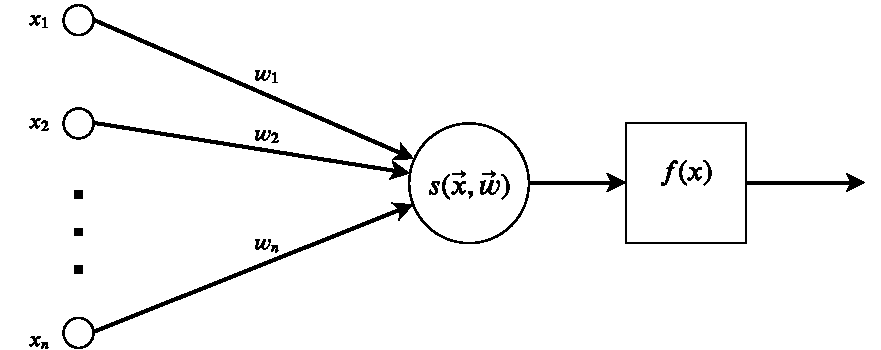
\includegraphics[scale=0.7]{Neuron.pdf}
\caption{Prikazani osnovni dijelovi neurona su težine dendrita ($w_i$), ulazna funkcija ($a(\vec{x},\vec{w})$) i izlazna funkcija ($f(x)$). Prag neurona nije prikazan zbog jednostavnosti dijagrama.}
\label{fig:neuron}
\end{figure}

Način na koji iz ulaza gradimo unutarnje stanje neurona opisujemo ulaznom funkcijom. Pretvorbu unutarnjeg stanja neurona u izlazni signal opisujemo izlaznom funkcijom koja se detaljnije obrađuje u poglavlju \ref{sec:izlazne_fje}. Ulazna i izlazna funkcija definiraju prijenosnu funkciju koja ujedno opisuje ponašanje cijelog neurona. Pojam prijenosne funkcije je potreban jer ih ponekad ne možemo podijeliti na ulazne i izlazne. Izlaznu funkciju ne treba miješati s funkcijom izlaza mreže koja predstavlja nelinearnost posljednjeg sloja mreže. U literaturi se umjesto pojma izlazne funkcije vrlo često koristi pojam aktivacijske funkcije. No u preglednim znanstvenim radovima \citep{function_survey1, function_survey2, function_survey3} pojam aktivacijske funkcije predstavlja ulaznu funkciju, što je neispravno sa stajališta teorijske neuroznanosti jer aktivacija neurona označava pojavu odaslanog signala iz some u akson \citep[p.~234]{neuroscience}. U starijoj literaturi je pojam aktivacijske i prijenosne funkcije često ekvivalentno korišten. S obzirom na nekonzistencije u literaturi i iz potrebe razlikovanja funkcija koje prikupljaju i odašilju signale iz neurona u ovom se radu koristi prvo navedena nomenklatura (ulazna, izlazna i prijenosna funkcija).
\begin{equation}
t(x) = (f \circ a)(x) = f(a(x))
\end{equation}

Najpopularnije ulazne funkcije jesu afina funkcija i unakrsna korelacija.
Afina funkcija je skalarni produkt vektora ulaza s vektorom težina neurona uz dodatak vrijednosti praga. Parametri neurona definiraju nagib i pomak ravnine u prostoru ulaza koja opisuje ulaz neurona. Primijenjuje se kada se ulazi u model mogu zapisati vektorom značajki čiji raspored nije bitan.
\begin{equation}
f(\vec{x};\mat{W},\vec{b})=\mat{W}^T \cdot \vec{x} + \vec{b}
\end{equation}

Unakrsna korelacija, za razliku od afine funkcije, koristi informaciju o susjednosti ulaznih značajki. Ulaz za takav model je definiran n-dimenzijskim tenzorom, a neuron uzima samo jednu regiju tenzora (vidljivu regiju) i nad njime računa skalarni produkt s n-dimenzijskim tenzorom parametara (jezgrom). Kada su ulazi slike u boji ulazni tenzor ima 3 dimenzije (visina, širina i RGB kanali) pa stoga i svaka jezgra ima 3 dimenzije, no znantno manje visine i širine. Unakrsna korelacija prozvana je konvolucijom jer radi na istom principu, a jedina razlika je da se elementi jezgre indeksiraju zrcaljeno po obje osi. S obzirom da se parametri jezgre uče automatski, nije nam bitno definirati orijentaciju jezgre. Unakrsna korelacija koristi iste parametre za svaku vidljivu regiju što ju čini štedljivijom od afine funkcije te ostvaruje neosjetljivost na translaciju, što je vrlo korisno u računalnom vidu.
\begin{equation}
f(\mat{X};\mat{W})=\mat{X} \circledast \mat{W}
\end{equation}

\todo{Je li uopće potrebno spominjat konvoluciju?}

Postoje i aktivacijske funkcije temeljene na udaljenosti vektora ...

\todo{Spomeni distance based aktivacije (ANFIS?)}
\todo{Spomeni i složenije metode: \citep{network_in_network}}

Povezivanjem neurona gradi se arhitektura mreže koja određuje kako podatci i gradijenti teku kroz mrežu, a time utječu na brzinu učenja i inferencije neuronske mreže. Najčešće se koriste slojevite unaprijedne arhitekture zbog jednostavnosti izvedbe. Unaprijedne arhitekture propuštaju podatke samo u jednom smjeru odnosno već izračunati neuroni se ne izračunavaju ponovno, što je posebno pogodno za optimizaciju širenjem unatrag, detaljnije opisanu u poglavlju \ref{sec:backprop}. Slojevite arhitekture omogućuju paralelizaciju izvođenja operacija na grafičkim karticama što značajno ubrzava postupke učenja i inferencije. Pri definiciji slojevite arhitekture najčešće je dovoljno navesti samo redoslijed slojeva, no ponekad je potrebno definirati i način povezivanja slojeva npr. pri uporabi preskočnih veza \citep{highwaynet, resnet, densenet}. Prvi sloj služi za postavljanje ulaza mreže i nazivamo ga ulaznim slojem mreže. Posljednji sloj mreže služi nam za ekstrakciju izlaza te mjerenje kakvoće mreže i nazivamo ga izlaznim slojem mreže. Svi slojevi između ulaznog i izlaznog sloja nazivaju se skrivenim slojevima.

Potpuno povezana arhitektura je najjednostavnija arhitektura za zadatak klasifikacije. Svaki neuron u potpuno povezanom sloju aktivira se pomoću svih izlaza iz prethodnog sloja. Za naučeni potpuno povezani sloj kažemo da vrši ekstrakciju značajki iz svojih ulaza. Geometrijski gledano, svaki neuron vrši mapiranje značajki iz dimenzije prethodnog sloja u novu dimenziju s ciljem modeliranja boljih značajki.

\todo{Daj neki dokaz za ovo gore.}

\subsection{Optimizacija umjetne neuronske mreže}
Optimizacijom parametara neuronska mreža prilagođava se danom zadatku, odnosno kažemo da mreža 'uči'. Optimizaciju parametara najčešće izvodimo gradijentnim spustom, uz pretpostavku derivabilnosti svih komponenata neuronske mreže. Kada ta pretpostavka ne vrijedi koriste se algoritmi kombinatorne optimizacije poput algoritma roja čestica koji se spominje u \citet{skripta_nenr}. U ovom radu neuronske mreže optimiraju se gradijentnim spustom.

\subsubsection{Gradijentni spust}
\label{sec:gradijentni_spust}

\todoimg{gradijentni spust unimodalna vs višemodalna (gdje preskoći brdo i uleti u bolji optimum)}
\label{fig:gradientni_spust}

Gradijentni spust je algoritam pronalaska minimuma funkcije vođen gradijentom te funkcije. Za zadanu početnu točku iterativno se pomiče u smjeru suprotnom od gradijenta funkcije u toj točki dok ne zadovolji neki od uvijeta zaustavljanja. Na strmim funkcijama gradijent je često prevelik i može izazvati oscilaciju ili divergenciju \figref{fig:oscilira_divergira}. Stoga se gradijent pri pomaku skalira koeficijentom pomaka $\mu$. Dobro odabran koeficijent pomaka može osigurati bržu konvergenciju, a kod višemodalnih funkcija i pronalazak boljeg optimuma \figref{fig:gradientni_spust}.

Početna točka utječe na ishod algoritma. Kod višemodalnih funkcija s optimumima različitih kvaliteta, početna točka može definirati u koji će lokalni optimum algoritam konvergirati \figref{fig:pocetna_tocka}.
\newline
\newline
\begin{algorithm}[H]
\KwIn{funkcija $f(\vec{x})$}
\KwIn{početna točka $\vec{x_0}$}
\KwIn{koeficijent pomaka $\eta$}
\KwIn{broj iteracija $n$}
\For{n iteracija}{
$\vec{g_i} \gets \vec{\nabla}_{\vec{x}} f(\vec{x_i})$ \;
$\vec{x_{i+1}} \gets \vec{x_i} - \eta \cdot \vec{g_i}$
}
\KwResult{konačna točka $\vec{x_i}$ je pronađeni optimum}
\caption{Gradijentni spust}
\label{alg:grad_spust}
\end{algorithm}

\todoimg{graidjentni spust stope spuštanja (velka, mala, taman)}
\label{fig:oscilira_divergira}

Broj iteracija definira koliko se puta pomičemo iz početne točke, što definira i trajanje algoritma. Generalno želimo skratiti vrijeme pretraživanja te povećati koeficijent spusta kako bismo koristili manje pomaka. No u praksi najčešće nailazimo na višemodalne funkcije sa strmim regijama koje izazivaju oscilacije i mogu izazvati divergenciju. Stoga se češće koriste manji pomaci kroz više iteracija. Dodatno se mogu dodati modifikacije gradijenta koje nude ograničavaju veličinu gradijenta (odsijecanje gradijenta i sl.).

\todoimg{gradijentni spust sa početnim točkama (jedna ode u lok, jedna ode u glob, jedna zapne desno na platou)}
\label{fig:pocetna_tocka}

Problem se javlja ako algoritam odluta u visoravan na kojoj su gradijenti vrlo mali, a sama regija je s obzirom na pomake ogromna \figref{fig:pocetna_tocka}. Kad gradijent postane neupotrebljivo malen kažemo da je \textit{iščeznuo}. U takvim slučajevima pomaže dodavanje momenta koji se akumulira kroz više iteracija i dodaje vektoru gradijenta. Kad algoritam naiđe na regiju s vrlo malim gradijentima, moment pokušava izvuči algoritam iz visoravni pomičući ga u smjeru koji je akumuliran. Kako moment ne bi izvukao algoritam iz optimuma, dodaje mu se koeficijent \textit{zaboravljanja} kojim se stari vektor momenta djelomično zaboravlja u korist novog vektora pomaka (jednadžba \ref{eq:moment_update}). Moment može pomoći i pri zaobilaženju lokalnih optimuma \figref{fig:pocetna_tocka}.

\begin{equation}
\label{eq:moment_update}
\begin{split}
\vec{v} &\gets \alpha \cdot \vec{v} - \eta \cdot \vec{g} \\
\vec{x} &\gets \vec{x} + \vec{v}
\end{split}
\end{equation}

\todoimg{moment prije i na visoravni, moment za savladavanje brda}
\label{fig:visoravan}

Algoritam je primijenjiv na funkcije proizvoljne dimenzionalnosti uz pretpostavku derivabilnosti u svakoj točki. Za proizvoljnu realnu funkciju, uz dobro odabrane hiperparametre, algoritam će konvergirati u jedan od lokalnih optimuma, no algoritam generalno nema garanciju konvergencije u globalni optimum. Garanciju pronalaska globalnog optimuma nudi jedino za trivijalne unimodalne funkcije uz odgovarajuće hiperparametre algoritma \figref{fig:gradientni_spust}.

Problem odabira hiperparametara proizlazi iz činjenice da u generalno praksi nemamo definiranu funkciju koju minimiziramo (već samo skup primjera te funkcije) i/ili ju ne možemo jasno vizualizirati (kada radimo s funkcijama visoke dimenzionalnosti). Čak i da imamo definiranu funkciju najčešće ne znamo koju vrijednost poprima globalni optimum, a pohlepna pretraga je netraktabilna. Unatoč tome, gradijentni spust efikasno i učinkovito pronalazi optimume koji su dovoljno dobri za većinu praktičnih primjena \citep{yolo}.

\subsubsection{Funkcija gubitka}
Pri učenju umjetnih neuronskih mreža potrebno je definirati funkciju gubitka. Funkcija gubitka, za dani ulaz, uspoređuje predikciju mreže sa željenim vrijednostima te dodjeljuje iznos pogreške (realan broj). Potrebno je pažljivo odabrati funkciju gubitka jer utječe na učenje svakog parametra (kao što je opisano u poglavlju \ref{sec:backprop}) te definira što je ishod učenja. 

Najčešće ne znamo definiciju funkcije gubitka na čitavoj promatranoj domeni već posjedujemo samo prijere te funkcije u podatcima koje smo izmjerili i koje smatramo reprezentativnim. Ovdje pretpostavljamo da će neuronska mreža ostvariti svojstvo generalizacije, koje je detaljnije objašnjeno u poglavlju \ref{sec:svojstva}. Stoga se u narednim formulama koristi notacija sumiranja.

Funkcija gubitka često je usko vezana uz vrstu problema koji se rješava (klasifikacija, regresija i ostali), način učenja (nadzirano, polu-nadzirano, nenadzirano, podržano) i izlaznu funkciju posljednjeg sloja neuronske mreže. U ovom radu vrši se klasifikacija nadziranim učenjem, no u nastavku se navodi i primjer funkcije gubitka za regresiju. Funkciju gubitka definiramo kao inverz funkcije izglednosti da neuronska mreža modelira funkciju predstavljenu primjerima podatkovnog skupa. Funkciju gubitka minimiziramo pa je definirana \textbf{negativnim logaritmom izglednosti} \eqref{eq:negloglikelyhood}. Logaritam je uveden zbog pojednostavljivanja distribucija koje sadrže eksponente.

\begin{equation}
\label{eq:negloglikelyhood}
L(\theta \probsep x,y) = -\log\ p(f(X;\theta)=y \probsep X=x)
\end{equation}

Zbog jednostavnosti zapisa, funkciju modela zapisujemo skraćeno kao aproksimaciju odnosno predikciju funkcije izlaza podatkovnog skupa te se ovisnost o ulazima podrazumijeva.
\begin{equation}
\hat{y} = f(x; \theta)
\end{equation}

 S obzirom da želimo procijeniti kvalitetu modela na čitavom podatkovnom skupu zanima nas očekivanje funkcije gubitka \eqref{eq:negloglikelyhood_expect}.
\begin{equation}
\label{eq:negloglikelyhood_expect}
\begin{split}
L(\theta \probsep \dataset) &= \expect_{(x,y) \sim p_\dataset}[L(\theta \probsep x,y)] \\
&= -\frac{1}{|\dataset|} \sum_{(x,y)\in\dataset} \log\ p(\hat{y}=y \probsep x)
\end{split}
\end{equation}

\textbf{U problemima regresije}, pretpostavlja se da izlazi mreže prate Gaussovu distribuciju s jediničnom kovarijacijskom matricom. Njenim uvrštavanjem u negativnu log. izglednost \eqref{eq:negloglikelyhood} dobivamo funkciju kvadratnog gubitka koja računa odstupanje izlaza neuronske mreže od željenih vrijednosti. Uz ovaj gubitak najčešće se koristi funkcija identiteta u izlaznom sloju.
\begin{align}
\label{eq:normal_dist}
\begin{split}
p(\hat{y}=y \probsep x) &= \normal(y \probsep \mu=\hat{y}, \mat{\Sigma}=\mat{I}) \\
&= \frac{1}{\sqrt{2\pi}\Sigma^{^1/_2}} \exp(-(y-\hat{y})^T\Sigma^{^1/_2}(y-\hat{y}))
\end{split}
\end{align}

Uvrštavanjem u \eqref{eq:negloglikelyhood} dobivamo kvadratni gubitak:

\begin{align}
\label{eq:loss_regression}
L(\theta \probsep x,y) &= - \log \Big[ \frac{1}{\sqrt{2\pi}\Sigma^{^1/_2}} \Big] - \log \Big[ \exp(-(y-\hat{y})^T\Sigma^{^1/_2}(y-\hat{y})) \Big] \nonumber \\
&= -\log c - (y-\hat{y})^T\Sigma^{^1/_2}(y-\hat{y}) \nonumber \\
&= \left|\footnotesize 
\begin{array}[c]{l} 
	c = konst. \\ 
	\Sigma = I 
\end{array}
\right| \nonumber \\
&= (y-\hat{y})^T(y-\hat{y}) = \sum_i (y_i - \hat{y}_i)^2
\end{align}

\textbf{U problemima klasifikacije}, pretpostavlja se da su izlazi mreže međusobno isključive slučajne varijable te stoga prate generaliziranu Bernoullijevu distribuciju (kategoričku distribuciju).
\begin{equation}
p(\hat{y}=y \probsep x) = \hat{y}_1^{y_1} \cdot \hat{y}_2^{y_2} \cdots \hat{y}_c^{y_c} 
= \prod_{i=1}^C \hat{y}_i^{y_i}, \quad \sum_i \hat{y}_i = 1
\end{equation}

Uvrštavanjem u \ref{eq:negloglikelyhood} dobivamo kategorički gubitak:
\begin{align}
\label{eq:loss_classification}
L(\theta \probsep x,y) &= - \log \Big[ \prod_{i=1}^C \hat{y}_i^{y_i} \Big] = - \sum_{i=1}^C y_i \log (\hat{y}_i)
\end{align}

\subsubsection{Optimizacija širenjem unatrag}
\label{sec:backprop}
Funkcija gubitka opisuje pogrešku čitave mreže te ovisi o svakom ugodljivom parametru mreže. Takva formulacija problema omogućuje nam da svaki parametrar mreže ugađamo gradijentnim spustom. Dakle, za parametriziranu funkciju $f(x;\theta)$ tražimo one parametre $\theta^*$ za koje je gubitak najmanji na podatkovnom skupu.
\begin{equation}
\theta^* = argmin_\theta\ L(\theta \probsep \dataset), \quad \forall (x,y) \in \dataset
\end{equation}

Optimiranje gradijentnim spustom zahtjeva derivabilnost funkcije koju optimiziramo po ulazima, što izrazi \eqref{eq:loss_regression} i \eqref{eq:loss_classification} zadovoljavaju. Pri tome koristi se pravilo ulančavanja parcijalne derivacije kompozicije funkcija.
\begin{equation}
\label{eq:partial_rule}
\dfrac{}{x} f(g(x)) = \pfrac{f(g(x))}{g(x)} \cdot \pfrac{g(x)}{x}
\end{equation}

Derivacijom funkcije gubitka za regresiju \eqref{eq:loss_regression} po ulazima, uz pretpostavku derivabilnosti čitave neuronske mreže po ulazima, dobivamo sljedeći izraz:
\begin{align}
\dfrac{L(\theta \probsep x,y)}{x} &= \dfrac{}{x}\sum_i(y_i - \hat{y}_i(x))^2 \nonumber \\
&= 2 \cdot \sum_i (y_i - \hat{y}_i(x)) \cdot \dfrac{\hat{y}_i(x)}{x}
\end{align}

Derivaciju funkcije gubitka za klasifikaciju možemo drastično pojednostaviti ako za izlaznu funkciju izlaznog sloja mreže odaberemo funkciju \textit{softmax} \eqref{eq:softmax_for_loss}, a izlaze kodiramo \textit{one-hot} oznakama \eqref{eq:onehot}. Ulaz u funkciju softmax su aktivacije neurona izlaznog sloja koje su ovdje označene vektorom $\vec{s}(x)$.
\begin{equation}
\label{eq:softmax_for_loss}
\hat{y}(\vec{x}) = \text{softmax}(\vec{s}(x)) = \frac{\exp(\vec{s}(x))}{\sum_{i=1}^{C} exp(s_i(x))}
%%% \quad \equiv \quad p(y_i \probsep x) = \frac{p(x|y_i)p(y_i)}{\sum_jp(x|y_j)p(y_j)}
\end{equation}

\begin{equation}
\label{eq:onehot}
\vec{y}=[y_1, y_2, \cdots, y_C], \quad y_i \in \{0,1\}, \quad \sum_{i=1}^C y_i = 1
\end{equation}

Uvrštavanjem u \eqref{eq:loss_classification} dobivamo:

\begin{align}
\label{eq:loss_classification_softmax}
L(\theta \probsep x,y) &= - \sum_{i=1}^C y_i \log \frac{\exp(s_i(x))}{\sum_{j=1}^{C} exp(s_j(x))} \nonumber \\
&= - \sum_{i=1}^C \bigg[ y_i \cdot s_i(x) - y_i \log\big(\sum_{j=1}^{C} exp(s_j(x))\big) \bigg] \nonumber \\
&= - \sum_{i=1}^C \big[ y_i \cdot s_i(x) \big] + \log\big[\sum_{j=1}^{C} exp(s_j(x))\big] \cdot \sum_{i=1}^C y_i \nonumber \\
&= \log\big[\sum_{j=1}^{C} exp(s_j(x))\big] - \sum_{i=1}^C \big[ y_i \cdot s_i(x) \big]
\end{align}

Derivacijom \eqref{eq:loss_classification_softmax} po ulazima, koristeći pravilo \eqref{eq:partial_rule} dobivamo:
\begin{align}
\dfrac{L(\theta \probsep x,y)}{x} &= \dfrac{L(\theta \probsep x,y)}{\vec{s}(x)} \cdot \dfrac{\vec{s}(x)}{x} \nonumber \\
&= \bigg[ \vec{s}(x) - y \bigg] \cdot \dfrac{s(x)}{x}
\end{align}



S obzirom da se mreža sastoji od ulančanih nelinearnih neurona s parametrima, gradijent gubitka moramo proslijediti sekvencijalno širenjem unazad (prema ulazima u mrežu). Pojedini neuron možemo smatrati parametriziranom funkcijom koju je moguće prikazati grafom \ref{fig:neuron_grad}. Vidimo da se ulazni gradijent prolaskom kroz neuron širi na ostale elemente i na ulaze neurona koji vode do prethodnih neurona. Primijetimo i da se širi u suprotnom smjeru od toka podataka. Iz toga proizlazi naziv "\textit{širenjem unazad}" \engl{backpropagation}.

\todoimg{neuron kao graf + tok gradijenata}
\label{fig:neuron_grad}

Želimo li učiti mrežu gradijentnim spustom, svaki parametar mreže treba imati pristup gradijentu funkcije gubitka. S obzirom da je neuron parametrizirana funkcija, pomoću koje ulančavanjem gradimo mrežu, dovoljno je pokazati da pojedini neuron osigurava svojim parametrima pristup gradijentu te da gradijent šalje svojim prethodnicima s kojima je povezan. Na slici \ref{fig:neuron_grad} vidimo da je to ostvarivo, što dokazuju i izrazi:
\begin{align}
\begin{split}
\pfrac{L(x,y;\theta)}{s(x;w)} &= \pfrac{L(x,y;\theta)}{o(x;w)} \cdot \pfrac{o(x;w)}{s(x;w)} \\
&= \pfrac{L(x,y;\theta)}{o(x;w)} \cdot f'(x)
\end{split}
\end{align}

\begin{align}
\begin{split}
\pfrac{L(x,y;\theta)}{x_i} &= \pfrac{L(x,y;\theta)}{s(x;w)} \cdot \pfrac{s(x;w)}{x_i} \\
&= \pfrac{L(x,y;\theta)}{o(x;w)} \cdot f'(x) \cdot w_i
\end{split}
\end{align}

\begin{align} \label{eq:w_update}
\begin{split}
\pfrac{L(x,y;\theta)}{w_i} &= \pfrac{L(x,y;\theta)}{s(x;w)} \cdot \pfrac{s(x;w)}{w_i} \\
&= \pfrac{L(x,y;\theta)}{o(x;w)} \cdot f'(x) \cdot x_i
\end{split}
\end{align}

\begin{align}
\begin{split}
\pfrac{L(x,y;\theta)}{w_0} &= \pfrac{L(x,y;\theta)}{s(x;w)} \cdot \pfrac{s(x;w)}{w_0} \\
&= \pfrac{L(x,y;\theta)}{o(x;w)} \cdot f'(x) \cdot 1
\end{split}
\end{align}

\subsubsection{Stohastički gradijentni spust}
U prošlom poglavlju koristili smo funkciju gubitka na jednom podatkovnom paru, no želimo minimizirati očekivanje funkcije gubitka \eqref{eq:negloglikelyhood_expect} na cijelom podatkovnom skupu jer želimo što preciznije procijeniti naš model i učit ga da aproksimira čitavu uzorkovanu funkciju što bolje. Nažalost, podatkovni skupovi poput spomenutog u poglavlju \ref{sec:dpa_datasets} vrlo su veliki i nije ih praktično koristiti pri optimizaciji gradijentom jer bismo ih čitave morali držati u brzoj memoriji. Ovo predstavlja velik problem pri računanju s grafičkim karticama. Očekivanje gubitka služi nam za procjenu smjera i veličine gradijenta. Ako gradijent procjenjujemo na čitavom podatkovnom skupu on će nas dovesti do prvog optimuma koji najčešće nije dobar, odnosno snažno ovisi o odabiru početne točke. 

S druge strane, ako gradijent računamo na pojedinom podatkovnom paru kao u \eqref{eq:loss_classification} ostvarili smo stohastičko kretanje jer će svaki primjer usjeriti gradijent u drugom smjeru. Posljedica toga je dulje vrijeme pretrage, no veća otpornost na loše lokalne optimume. Iako će algoritam generalno konvergirati, postupak je zahtjevan jer za svaki primjer podatkovnog skupa trebamo provesti korak algoritma. Ovaj problem također ograničava svojstvo ubrzanja grafičkim karticama koje nude masivnu paralelizaciju operacija nad podatcima.

Iz navedenih razloga želimo vršiti procjenu gradijenta na "nekoliko" primjera. Podskup takvih primjera nazivamo \textbf{mini-grupom} \engl{mini-batch}. Najčešće se uzima najveći broj primjera koji grafička kartica može efikasno obraditi i koji je potencija broja 2. Mini-grupe i dalje zadržavaju stohastičnost kretanja gradijenta (posebice ako je veličina manja od broja klasa), ali procjenjuju bolje od potpuno stohastičnog te brže konvergiraju. Sada formula \eqref{eq:negloglikelyhood_expect} poprima oblik koji odgovara očekivanju pojedine mini-grupe $\minibatch_i$.
\begin{equation}
\label{eq:negloglikelyhood_expect}
\begin{split}
L(\theta \probsep \dataset) &= \expect_{(x,y) \sim p_{\minibatch_i}}[L(\theta \probsep x,y)] \\
&= -\frac{1}{|\minibatch_i|} \sum_{(x,y)\in\minibatch_i} \log\ p(\hat{y}=y \probsep x)
\end{split}
\end{equation}

Mini-grupe se najčešće definiraju prije početka učenja nasumičnim rasporedom. To je najjednostavniji i najbrži pristup, no definiranjem fiksnih mini-grupa unosi induktivnu pristranost jer ne možemo znati je li odabran raspored idealan za model koji evaluiramo. Pristranost možemo ublažiti miješanjem podatkovnog skupa između epoha, no skupocijenost te operacije ograničava njeno korištenje u praksi. Također, problem mogu stvoriti mini-grupe pristrane jednoj ili više dominantnih (većinskih) klasa koje će snažno usmjeravati gradijent prema tim klasama i zanemarivati ostale. Taj problem je posebno izražen u nebalansiranim podatkovnim skupovima, a može se zaobići tehnikom težinskog uzorkovanja s ponavljanjem gdje je vjerojatnost odabira primjera obrnuto proporcionalna dominantnosti (brojnosti) njegove klase. Treba paziti da se provede dovoljan broj uzorkovanja tako da je model učen na svakom primjeru podatkovnog skupa.

\begin{algorithm}[H]
\KwIn{funkcija $f(\vec{x})$}
\KwIn{inicijalizirani parametar $\theta_0$}
\KwIn{stopa učenja $\eta$}
\KwIn{kriterij zaustavljanja $k$}
\While{kriterij $k$ nije zadovoljen}{
	\For{$\minibatch_i \in \dataset$}{
		$\vec{g_i} \gets \frac{1}{|\minibatch|} \sum_{(\vec{x},\vec{y})\in\minibatch} \vec{\nabla}_{\theta} L(\theta \probsep \vec{x},\vec{y})$ \;
		$\vec{\theta_{i+1}} \gets \vec{\theta_i} - \eta \cdot \vec{g_i}$
	}
}
\caption{Stohastički gradijentni spust}
\label{alg:sgd}
\end{algorithm}

\subsubsection{Optimizator}
Optimizator brine o pomaku odnosno ažuriranju parametara modela pri gradijentnom spustu. Dosad smo vidjeli dva načina: klasični s koeficijentom pomaka (algoritam \ref{alg:grad_spust}) i s dodatkom momenta \eqref{eq:moment_update}. Moment 

\todo{uporaba momenta i momenta na kvadrat (interpretacija)}
\todo{Adam}

\subsubsection{Promijenjiva stopa učenja}
Tijekom optimizacije gradijentnim spustom uz fiksnu stupu učenja optimizacija će početi oscilirati. Oscilacija se javlja kada je funkcija gubitka generalno konveksna po regijama, no sadrži 

\todo{zašto je problem u stopi}
\todo{zbog nekonveksnih izbočina tam dolje, stopa može biti prejaka}
\todoimg{konveksasta fja u kojoj skok u višljim regijama stvara manje problema od skokova u nižim}

Jedan način smanjivanja stope je zadavanje ključnih iteracija u kojima se prestaje koristiti stara stopa i koristi se nova. Moguće je zadati stope za svaku od zadanih ključnih iteracija \citep{onaj rad} ili zadati početnu stopu koja se u ključnoj iteraciji pomnoži konstantom manjom od 1. Pri ovom pristupu problem je odrediti optimalne ključne iteracije ili početnu iteraciju i konstantu.

Ključnim iteracijama možemo proglasiti one u kojima je detektirana konvergencija ili divergencija. Taj pristup omogućava nastavak pretrage, no problem je kako sa sigurnošću detektirati konvergenciju ili divergenciju. Tipično učenje mreže nije monotono, tj. gubitak mreže može na neko vrijeme rasti prije no što nastavi padati, što odgovara ponašanju u lokalnom optimumu. U tom slučaju smanjivanje stope učenja je nepoželjno.

\todo{WTF??? Zašto bi itko smanjivao stopu? jel zato kaj je oštrina brda tam dolje opasna za malu regiju koju pretražujemo? wtf?}
\todo{zašto bi loss rastao?}

Pristup koji se koristi u ovom radu, je zadati početnu stopu i u svakoj iteraciji pomnožiti ju s konstantom manjom od 1. Pri tome se ne pretpostavlja postojanje ključnih iteracija i stopa se konstantno smanjuje. Uz korištenje stohastičkog gradijentnog spusta postupak navodi pretragu na sve finije regije funkcije gubitka. Postupak povlači slićnost s postupkom simuliranog kaljenja gdje se smanjivanjem temperature sustava smanjuje njegova stohastičnost i postupak konvergira u sve finije regije rješenja.

\todo{postoji množenje faktorom pri detekciji konvergencije, ali ne želim ga jer ne znam kada konvergira (stepeničasto učenje)}

\subsubsection{Inicijalizacija parametara}
Inicijalizacija parametara mreže odgovara odabiru početne točke pri gradijentnom spustu. Dobrom inicijalizacijom možemo osigurati pronalazak boljeg optimuma te u kritičnim slučajevima i osigurati konvergenciju mreže. S obzirom da neuronske mreže posjeduju jasnu strukturu (što je posebno izraženo u slojevitim arhitekturama) inicijalizacija ima dodatne utjecaje. U potpuno povezanim slojevima želimo da svaki neuron vrši ekstrakciju značajki. Pri tome, u efikasnom sloju svaki će neuron stvoriti svoju značajku. Ako je više neurona inicijalizirano dovoljno slićno, ti neuroni će naučiti izvlaćiti iste značajke. Kažemo da je došlo do \textbf{koadaptacije neurona}.

Inicijalizacija slojevitim nenadziranim učenjem ograničenog Boltzmann-ovog stroja \engl{restricted Boltzmann machine} pokazuje se dobrom \citep{relu6}. Postupak nenadzirano trenira stohastičku mrežu sloj po sloj na ulaznim značajkama kako bi slojevi ostvarili dobru ekstrakciju viših značajki. Nakon treniranja, mreži se dodaje izlazni klasifikacijski sloj i mreža se nadzirano ugađa na skupu za učenje. Iako je ostvarena inicijalizacija vrlo dobra, postupak je vremenski zahtjevan. Uvođenjem 

\todo{važnost dobre inicijalizacije}
\todo{Xavier}
\todo{postoji i init. autoenkoderom, ali u kontekstu evolucije je preskupa}

\subsubsection{Pretprocesiranje podataka}
\todo{normalizacija po značajkama}
Koeficijenti se računaju pomoću značajki iz podatkovnog skupa za učenje. Koeficijent varijance ovisi o koeficijentu sredine pa se njihovo računanje ne može paralelizirati.
\begin{equation}
\vec{\mu} = \frac{1}{N} \sum_{\vec{x}\in \dataset} \vec{x}
\end{equation}
\begin{equation}
\vec{\sigma^2} = \frac{1}{N-1} \sum_{\vec{x}\in \dataset} (\vec{x}-\vec{\mu})^2
\end{equation}

Prije no što model dobije ulazne značajke, normaliziramo ih formulom:
\begin{equation}
\vec{z} = \frac{\vec{x} - \vec{\mu}}{\vec{\sigma^2}}
\end{equation}

Koeficijenti normalizacije se računaju samo na skupu za učenje, a normalizacija se mora primijeniti prilikom inferencije odnosno na skupu za testiranje.
\todoimg{slika značajki prije i poslije normalizacije}
\todo{sada su vrijednosti centriranje sa std.dev.}

\subsection{Regularizacija}
\label{sec:regularizacija}
Decizijska granica je sjecište 

\todo{geometrijski opis deciziske granice}

Podatkovni skupovi najčešće sadrže šum zbog nesavršenog uzorkovanja stvarne funkcije, pogrešnog označavanja ili višeznačnosti primjera. Bez regularizacije, model će s ciljem minimiziranja gubitka svoju decizijsku granicu saviti kako bi što ispravnije obuhvatio sve primjere pa čak i šum. Tada kažemo da je model počeo učiti šum odnosno da je \textbf{prenaučen}.

\todo{podnaučena, generalizira, prenaučena}
\todoimg{podnaučena, generalizira, prenaučena}

\subsubsection{Regularizacija parametara}
Prenaučenost je često posljedica velikih normi vektora parametara. Stoga se u funkciju gubitka dodaje regularizacijski član po težinama $\Omega(\theta)$. Utjecaj regularizacije moguće je mijenjati hiperparametrom $\alpha$.
\begin{equation}
\label{eq:weights_regularization}
\tilde{L}(\theta \probsep x,y) = L(\theta \probsep x,y) + \alpha\Omega(\theta)
\end{equation}

Najčešće se koristi regularizacija \textbf{L2} normom koja akumulira kvadrate svih parametara modela. Pri ažuriranju parametra formula dobiva skaliranu vrijednost tog parametra što smanjuje vrijednost negativnog gradijenta.
\begin{equation}
\Omega(\vec{\theta}) = \frac{1}{2} \|\vec{w}\|_2^2 = \frac{1}{2} \sum_i w_i^2
\end{equation}
\begin{equation}
\vec{\theta}_{i+1} \gets \vec{\theta}_i - \eta \cdot \vec{g}_i + \alpha \cdot \theta
\end{equation}

\todo{Spomeni pokoju još (L1, adversarial iz Hintona, ...)}

\subsubsection{Regularizacija šumom}
Unošenjem šuma u podatke netom prije nego ih dobije model moguće je graditi robusnost modela na šum, ali ujedno to sprječava model da se pretrenira na podatkovnom skupu za treniranje. Jedan primjer možemo nasumično zašumiti nekoliko puta te se time povećava efektivna veličina podatkovnog skupa.

U ovom se radu ne koristi regularizacija šumom jer bi mogla imati nepredvidivi utjecaj na učenje. Primjena na slike je vrlo jasna jer uz dovoljno malu amplitudu aditivnog šuma teksture na slici će ostati očuvane zahvaljujući susjedstvu piksela, odnosno izrezivanjem slike obrasci će ostati netaknuti. Značajke podatkovnih skupova navedenih u poglavlju \ref{sec:dpa_datasets} su PCA redukcije originalnih slijedova signala koji su ispunjeni šumom očitavanja.

\todo{ajd svejedno isprobaj, grafi za ljubav}

\subsubsection{Rano zaustavljanje}
Pri učenju modela funkcija gubitka na skupu za učenje i testiranje generalno opada, no u jednom trenu gubitak generalizacije počinje rasti. Zaustavimo li učenje u trenutku kada je gubitak generalizacije najmanji dobili smo optimalan model za zadane hiperparametre. U praksi te funkcije neće biti naročito glatke zbog stohastičkog gradijentnog spusta te greška će generalizacije povremeno i rasti kako savladava lokalne optimume.

Postupak ranog zaustavljanja tretira broj epoha kao hiperparametar koji se pretražuje po liniji. No umjesto da za svaku vrijednost broja epoha nanovo treniramo model, ovdje ga treniramo jednom i jednostavno odaberemo vrijednost za koju model generalizira najbolje. To upućuje na potrebu krosvalidacije koja je opisana u poglavlju \ref{sec:crossval}.

\todoeq{Algoritam ranog zaustavljanja}

\subsection{Odabir hiperparametara}
Do ovdje su navedeni hiperparametri koji se koriste pri spomenutim tehnikama optimizacije neuronske mreže (poglavlja \ref{sec:gradijentni_spust} - \ref{sec:regularizacija}). No neuronska mreža ima i strukturalne hiperparametre.

Arhitektura mreže je vrlo bitan hiperparametar koji određuje složenost modela te utječe na brzinu inferencije i učenja modela. Razvijene su razne arhitekture koje koriste preskočne veze za postizanje vrlo dubokih arhitektura \citep{resnet, densenet}. Preskočne veze omogućavaju direktniji prijenos gradijenta što pomaže kod problema iščezavajućeg gradijenta u dubokim mrežama (poglavlje \ref{sec:iscezavajuci_grad}). Arhitektura može omogućiti dodatnu paralelizaciju inferencije i učenja tako da se teške operacije raspodijele na više uređaja, a rezultati spoje samo kada je to nužno \citep{alexnet}.

Izlazne funkcije su također važan hiperparametar, no u praksi se većinom ignoriraju zbog manjka intuicije o njihovom utjecaju na učenje pojedinog modela na pojedinom podatkovnom skupu. U praksi se najčešće odabiru funkcije koje su brze i koje se pokazuju korisnima u raznim radovima. Najčešće se koristi ReLU opisan u poglavlju \ref{func:relu}. U povratnim neuronskim mrežama za rekurzivne slojeve popularan je tangens hiperbolni opisan u poglavlju \ref{func:tanh}. U poglavlju \ref{sec:izlazne_fje} navedene su i opisane brojne funkcije te je njihov utjecaj ispitan u poglavlju \ref{sec:rezultati}.

\subsubsection{Procjena generalizacije i odabir modela}
Skup podataka kojim učimo model najčešće ne opisuje stvarnu funkciju potpuno, već sadrži primjere koje smatramo reprezentativnim i koji su dovoljni za njeno modeliranje. Kako bismo procjenili koliko dobro naš model procjenjuje stvarnu funkciju ispitujemo model na podatcima koji nisu korišteni prilikom učenja, odnosno na neviđenim podatcima. Ta se metoda zove \textbf{unakrsna validacija}, a skupove nazivamo \textbf{skupom za učenje} i \textbf{skupom za testiranje}. Dakako, važno je pobrinuti se da su oba skupa reprezentativna stvarnoj funkciji, ali da ne sadrže iste primjere. U suprotnom mreža će naučiti pogrešnu funkciju što može dati lažno pesimistične rezultate ili ćemo nepotpuno ili pristrano testirati što može dovesti do lažno optimističnih rezultata.

Svojstvo modela da dobro modelira na neviđenim primjerima naziva se generalizacija i detaljnije je opisano u poglavlju \ref{sec:generalizacija}. Pri odabiru hiperparametara ili pri odabiru modela potrebno je usporediti generalizaciju svakog pomoću zajedničke mjere. U problemima regresije najčešće se koristi ukupna vrijednost funkcije gubitka na čitavom skupu za testiranje.

\begin{equation}
\label{eq:mat_zabune_bin}
\begin{tabular}{|c|c|c|} \hline
\large{$_{\hat{y}} \setminus ^y$} & $\top$ & $\bot$ \\ \hline
$\top$	& TP & FP \\ \hline
$\bot$	& FN & TN \\ \hline
\end{tabular}
\end{equation}

Pri \textbf{binarnoj klasifikaciji} definiramo \textbf{matricu zabune} \eqref{eq:mat_zabune_bin} koja sadrži četiri elementa \eqref{eq:true_groups} koji definiraju vrstu pogodka i pogreške.
\begin{align}
\label{eq:true_groups}
\begin{split}
\text{Stvarno pozitivni:} \quad TP &= \sum_{(x,y)\in\mathbb{D}} \mathbbm{1} \{h(x) = \top \wedge y = \top \} \\
\text{Stvarno negativni:} \quad TN &= \sum_{(x,y)\in\mathbb{D}} \mathbbm{1} \{h(x) = \bot \wedge y = \bot \} \\
\text{Lažno pozitivni:}   \quad FP &= \sum_{(x,y)\in\mathbb{D}} \mathbbm{1} \{h(x) = \top \wedge y = \bot \} \\
\text{Lažno negativni:}   \quad FN &= \sum_{(x,y)\in\mathbb{D}} \mathbbm{1} \{h(x) = \bot \wedge y = \top \}
\end{split}
\end{align}

Iz tih skupova tada gradimo složenije mjere. \textbf{Točnost} je mjera kojom iskazujemo postotak točno pogođenih primjera:
\begin{equation}
Acc = \frac{TP+TN}{TP+TN+FP+FN}
\end{equation}

Točnost je dobra mjera, no samo ako je brojnost klasa u podatkovnom skupu balansiran. Ako je brojnost jedne klase puno veća od druge tada će trivijalan klasifikator, koji sve primjere klasificira u tu klasu, davati veliku točnost i razlika naspram ispravnijeg klasifikatora biti će nezamjetna. Stoga se kod nebalansiranih setova češće koristi \textbf{\F1 mjera}, koja uzima u obzir \textbf{preciznost} klasifikatora u razlikovanju pozitivnih primjera od negativnih \eqref{eq:precision} i njegov \textbf{odziv} odnosno obuhvat svih pozitivnih primjera testnog skupa \eqref{eq:recall}. \F1 mjera je definirana kao hamonijska sredina između preciznosti i odziva \eqref{eq:f_measure}. Postoji i generalizirana mjera F$_\beta$ koja dodjeljuje veću težinu preciznosti ili odzivu \eqref{eq:f_beta}, no u ovom radu koristi se samo \F1 koja pridijeljuje jednaku težinu. Harmonijska sredina se koristi jer je najstroža između Pitagorinih mjera za sredinu kao što prokazuje slika \ref{fig:sredine}.
\begin{align}
\text{Preciznost:} \quad P &= \frac{TP}{TP+FP} \label{eq:precision} \\
\text{Odziv:} \quad R &= \frac{TP}{TP+FN} \label{eq:recall} \\
\text{F}_1: \quad F_1 &= 2 \cdot \frac{P \cdot R}{P + R} \label{eq:f_measure} \\
\text{F}_\beta: \quad F_\beta &= (1 + \beta^2) \cdot \frac{P \cdot R}{\beta ^2 \cdot P + R} \label{eq:f_beta}
\end{align}

\begin{figure}[h]
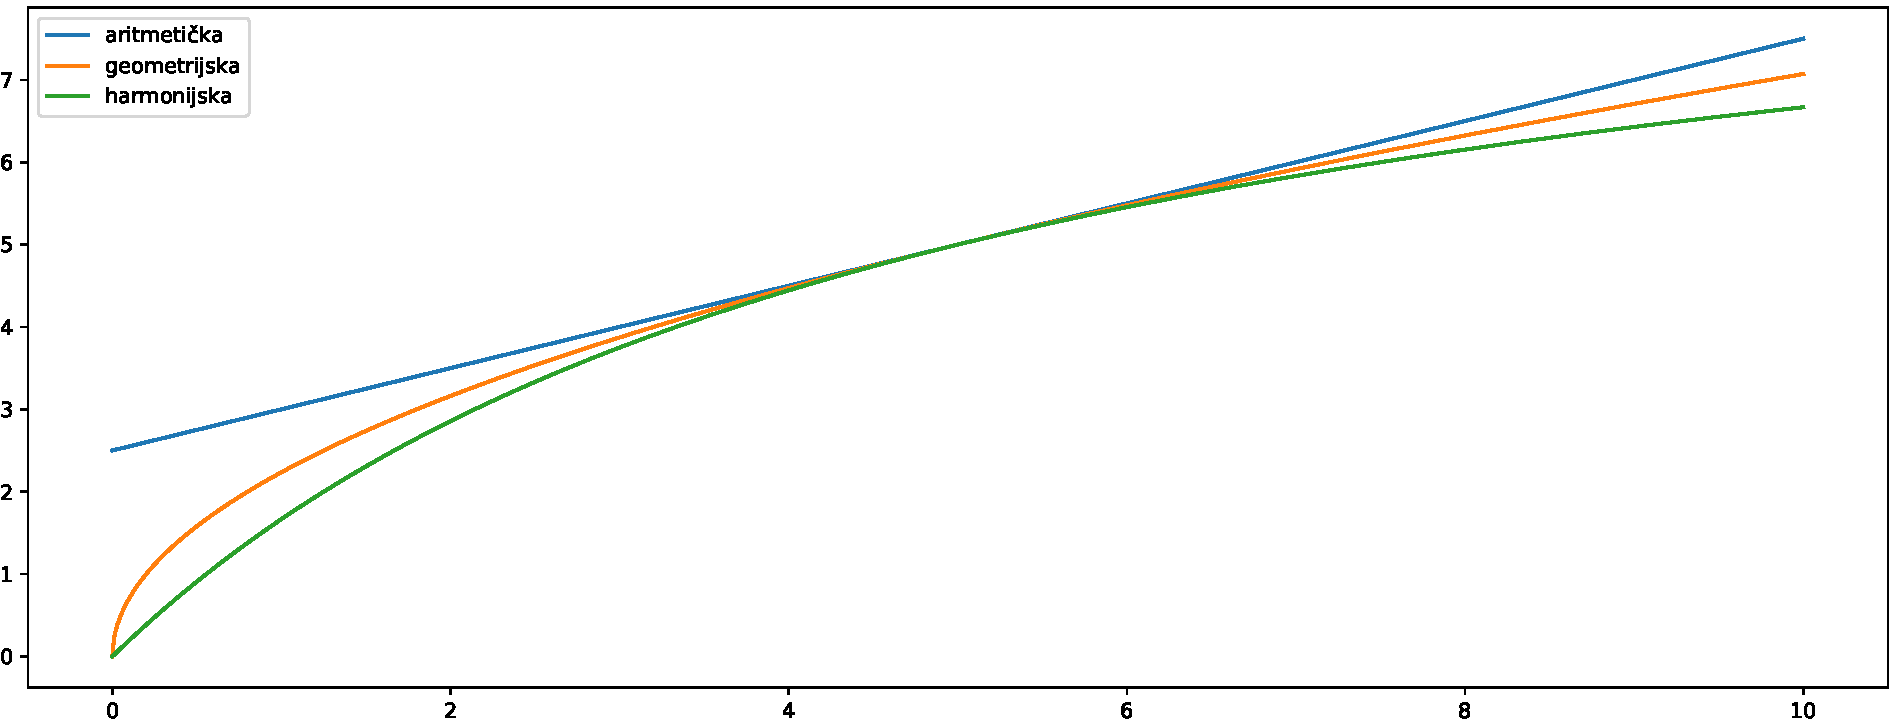
\includegraphics[width=\textwidth]{Pitagorine_sredine.pdf}
\centering
\caption{Pitagorine mjere za sredinu između dviju vrijednosti}
\label{fig:sredine}
\end{figure}

Mjere binarne klasifikacije možemo primijeniti pri \textbf{višeklasnoj klasifikaciji}, no matrica zabune je dimenzija $C\times C$ gdje je $C$ broj klasa. Elementi matrice računaju se slično kao i kod binarne klasifikacije, ali za svaku klasu posebno.
\begin{align}
\label{eq:true_groups}
\begin{split}
\text{Stvarno pozitivni:} \quad TP_i &= \sum_{(x,y)\in\mathbb{D}} \mathbbm{1} \{h(x) =  C_i \wedge y = C_i \} \\
\text{Stvarno negativni:} \quad TN_i &= \sum_{(x,y)\in\mathbb{D}} \mathbbm{1} \{h(x) \neq C_i \wedge y \neq C_i \} \\
\text{Lažno pozitivni:} \quad FP_i &= \sum_{(x,y)\in\mathbb{D}} \mathbbm{1} \{h(x) = C_i \wedge y \neq C_i \} \\
\text{Lažno negativni:} \quad FN_i &= \sum_{(x,y)\in\mathbb{D}} \mathbbm{1} \{h(x) \neq C_i \wedge y = C_i \}
\end{split}
\end{align}

Za izračun složenijih mjera poput točnosti i \F1 mjere moramo računati prosjek po klasama. Razlikujemo dva pristupa računanju prosjeka: makro i mikro. \textbf{Makro prosjekom} se prvo izračunaju mjere svake klase naspram svih ostalih te se uzme njihov prosjek. Ova mjera pretpostavlja jednak utjecaj svih klasa nez obzira na njihovu veličinu \citep{ml_probabilistic}.
\begin{equation}
\begin{split}
Acc^M = \sum_{i=1}^K \frac{Acc_i}{K}
\end{split} \quad
\begin{split}
P^M = \sum_{i=1}^K \frac{P_i}{K}
\end{split} \quad
\begin{split}
R^M = \sum_{i=1}^K \frac{R_i}{K}
\end{split} \quad
\begin{split}
F_1^M = \sum_{i=1}^K \frac{F_{1;i}}{K}
\end{split}
\end{equation}

\textbf{Mikro prosjekom} se prvo zbroje matrice zabune po pojedinim klasama, a zatim se nad zbrojenom matricom računaju mjere. Na mikro prosjek više utječe veličina klasa i koristi se u nebalansiranim skupovima.

\begin{align}
\begin{split}
Acc^\mu &= \frac{\sum_i (TP_i+TN_i)}{\sum_i (TP_i+TN_i+FP_i+FN_i)} = Acc^M \\
FP = FN \implies P^\mu &= R^\mu = F_1^\mu = \frac{\sum_i TP_i}{\sum_i (TP_i+FP_i)}
\end{split}
\end{align}

\subsubsection{Krosvalidacija}
\label{sec:crossval}
\todo{ovo je bitno}
... pri ćemu se skup za učenje podijeli na manji skup za učenje i skup za validaciju. Tek nakon što otkrijemo optimalan broj epoha model trenira na čitavom skupu za učenje i ispituje na skupu za testiranje koji mjeri stvarnu generalizaciju.

\subsubsection{Pretraživanje po rešetci}
\label{sec:grid_search}
Najjednostavniji način za pretraživanje hiperparametara je pretraživanje po rešetci. Za svaki hiperparametar koji optimiziramo definiramo vrijednosti koje želimo ispitati. Algoritam tada evaluira dani model za svaku kombinaciju hiperparametara i vraća kombinaciju ili model koji ostvaruje najbolje rezultate.

Iako se optimalni hipermarametri mogu nalaziti izvan zadanih skupova i neće biti pronađeni, postupak je brz i daje dovoljno dobre rezultate za praktičnu primjenu. Često je dovoljno da pronađe kombinaciju hiperparametara za koju model ne divergira niti prestaje učiti određen broj iteracija.

\subsection{Svojstva}
\label{sec:svojstva}

\subsubsection{Univerzalna aproksimacija}
Teorem univerzalne aproksimacije tvrdi da unaprijedna neuronska mreža može modelirati proizvoljnu Borel mjerljivu funkcju proizvoljno dobro uz nekoliko uvijeta: mora imati linearni izlaz, barem jedan nelinearni skriveni sloj koji koristi sažimajuću funkciju i "dovoljan" broj skrivenih neurona. Dakle, postoji arhitektura i postoje parametri kojima neuronska mreža može modelirati zadani podatkovni skup. No, teorem ne iskazuje kako doći do tih parametara što optimizaciju neuronske mreže čini vrlo teškom \citep{goodfellowbook}. 

\subsubsection{Dubina}
Iako je prema teoremu univerzalne aproksimacije dovoljan jedan nelinearni skriveni sloj za predstavljanje proizvoljne Borel mjerljive funkcije, gornja granica veličine tog sloja je eksponencijalno velika naspram broja ulaza što je netraktabilno. Dodavanjem dubine moguće je iskoristiti pravilnosti u funkciji koju aproksimiramo kako bismo smanjili potreban broj neurona. Primjer su funkcije simetrične oko neke osi. Ako skriveni slojevi mreže vrše preklapanje te funkcije preko same sebe, uzastopnim preklapanjem dobiva se sve jednostavnija funkcija. Preklapanje mogu vršiti po-dijelovima-linearne izlazne funkcije poput ReLU i Maxout. Dakako, ne postoji garancija da stvarna funkcija zadovoljava svojstvo simetrije, no u praksi dublje mreže generaliziraju bolje \citep{alexnet, highwaynet, resnet, densenet}. Postoje i druge interpretacije utjecaja dubine, poput svojstva dekompozicije zadatka na manje cjeline ili interpretacija neuronske mreže ako računalnog programa koje nadilaze temu ovog rada \citep{goodfellowbook}.

\todo{VC dimenzija}

\subsubsection{Kompresija}
\todo{kompresija}
\todo{https://www.quantamagazine.org/new-theory-cracks-open-the-black-box-of-deep-learning-20170921/}

\subsubsection{Generalizacija}
\label{sec:generalizacija}
\todoimg{underfit-fit-overfit}
\todo{generalizacija}
\todoimg{train-test U curve}

Ovo je posebno izraženo kod klasifikacije slika gdje za jednu generičku klasu (npr. automobil) postoji neprebrojivo mogućih slika s različitim modelom, bojom ili kutom gledanja automobila. No mi raspolažemo sa svega nekoliko stotina tisuća primjera koje smatramo reprezentativnim za tu klasu i želimo izgraditi klasifikator koji je robustan na većinu perturbacija slike.

\todo{negdje spomeni da su neuralke zapravo vrlo ograničene jer ograničavamo prostor mogućnosti zadavanjem fiksnih izlaznih fja, arhitekture i načina optimizacije (induktivna pristranost ograničavanjem skupa hipoteza). leži negdje između GP i ručno izgrađenih modela (jer je neuralka samo stablo funkcija kao u TF). CGP unosi ograničenje strukture što je bliže neuralki i daje zanimljive rezultate (atari cgp). Čini se da im godi balans između strukture i nasumičnosti.}

\subsection{Problemi}
\subsubsection{Odabir hiperparametara}
Arhitektura, prijenosne funkcije i parametri definiraju neuronsku mrežu te njihov pravilan odabir značajno utjeće na performanse neuronske mreže. Nažalost nije ih moguće optimalno odabrati u zatvorenom obliku, već se to svodi na problem pretraživanja kao što je pretraživanje po rešetci \ref{sec:grid_search}. Arhitekture mogu poprimiti vrlo složene oblike kao što je predstavljeno radovima \citet{highway}, \citet{resnet}, \citet{densenet}, \citet{inceptionnet} i \citet{yolo} te se najčešće grade ručno s maksimalnom traktabilnom složenošću mreže. Detaljnije o odabiru izlaznih funkcija napisano je u poglavlju \ref{sec:izlazne_fje}.

\subsubsection{Isčezavajući gradijent}
\label{sec:iscezavajuci_grad}
\todo{Problem dubokih arhitektura}

\subsubsection{Pretreniranost i neprijateljski primjeri}
\todo{Problem pretreniranosti + neprijateljski primjeri}

Derivabilne neuronske mreže optimiziraju se optimizatorom koji određuje kako se mijenjaju parametri. Za ugađanje parametara najčešće se koristi gradijentni spust, uz pretpostavku derivabilnosti čitave neuronske mreže. Kada pretpostavka ne vrijedi najčešće se koriste evolucijski algoritmi.

\chapter{Izlazne funkcije}
\label{sec:izlazne_fje}
Izlazna funkcija služi unošenju nelinearnosti u neuronsku mrežu i ima utjecaj na njeno učenje. Prilikom inferencije izlazna funkcija stvara nelinearnosti u decizijskoj granici koje su parametrizirane parametrima neurona na koji se primijenjuje. U slojevitim arhitekturama izlazne funkcije se primijenjuju uzastopno s različitim parametrima i vrše nelinearne projekcije iz jedne dimenzije u drugu.

Prilikom učenja neuronske mreže važan nam je utjecaj derivacije izlazne funkcije na gradijent pri širenju unatrag. Prolaskom unazad gradijent se množi s parametrima slojeva koji se mogu zapisati matricom težina $\mat{W}$. Uzastopnom primijenom matrica težina, ako su loše kondicionirane, može doći do "\textit{isćezavanja}" ili "\textit{eksplozije}" gradijenta.

\section{Odabir izlazne funkcije}
Za odabir izlazne funkcije ne postoji jasno pravilo. U praksi se odabiru empirijski po pokazanim rezultatima i brzinom (te implementacijskom podrškom), s preferencijom onih koje imaju neka teorijski potkrijepljena svojstva.

\todo{Bitka za odabir izlazne fje (nađi onaj rad di pljuje po sigmoidi i relu (elu rad?))}

U radu \citet{elish} autori koriste simboličku regresiju kako bi izgradili dvodjelnu izlaznu funkciju, sa zasebnom funkcijom u negativnoj i pozitivnoj domeni te definiraju dvije ručno izgrađene funkcije. Pretražuju se funkcije koje su jednostavne kompozicije popularnih izlaznih funkcija s ciljem iskorištavanja njihovih dobrih svojstava. Funkcije se primijenjuju na duboke arhitekture ResNet56 i VGG16 i na nekoliko podatkovnih skupova: CIFAR-10, CIFAR-100 i Tiny-ImageNet. Rezultati pokazuju poboljšanje kompozicije u odnosu na popularne funkcije gdje pozitivan dio često sadrži linearnu komponentu, a oblikom funkcije podsjećaju na zglobnicu \figref{fig:relu}.

\subsection{Izlazne funkcije s učećim parametima}
\todo{članak: učeći parametri u fjama (onaj stari)}

U radu \citet{trained_func} autori istražuju učeće izlazne funkcije ...

U radu TAF...

\subsection{Periodičke izlazne funkcije}
\todo{članak: fourier mreža s periodičkim fjama}
\todo{Članak: taming the waves}
\todo{ostale reference iz taming the waves}

\section{Popularne izlazne funkcije}

U nastavku su navedene izlazne funkcije koje je autor pronašao u literaturi i koje su isprobane u ovom radu. Za svaku funkciju napisana je formula i iscrtan izgled funkcije i njene derivacije te navedena neka poznata svojstva.

\subsection{Funkcija identiteta}
\engl{Identity function}

\begin{figure}[H]
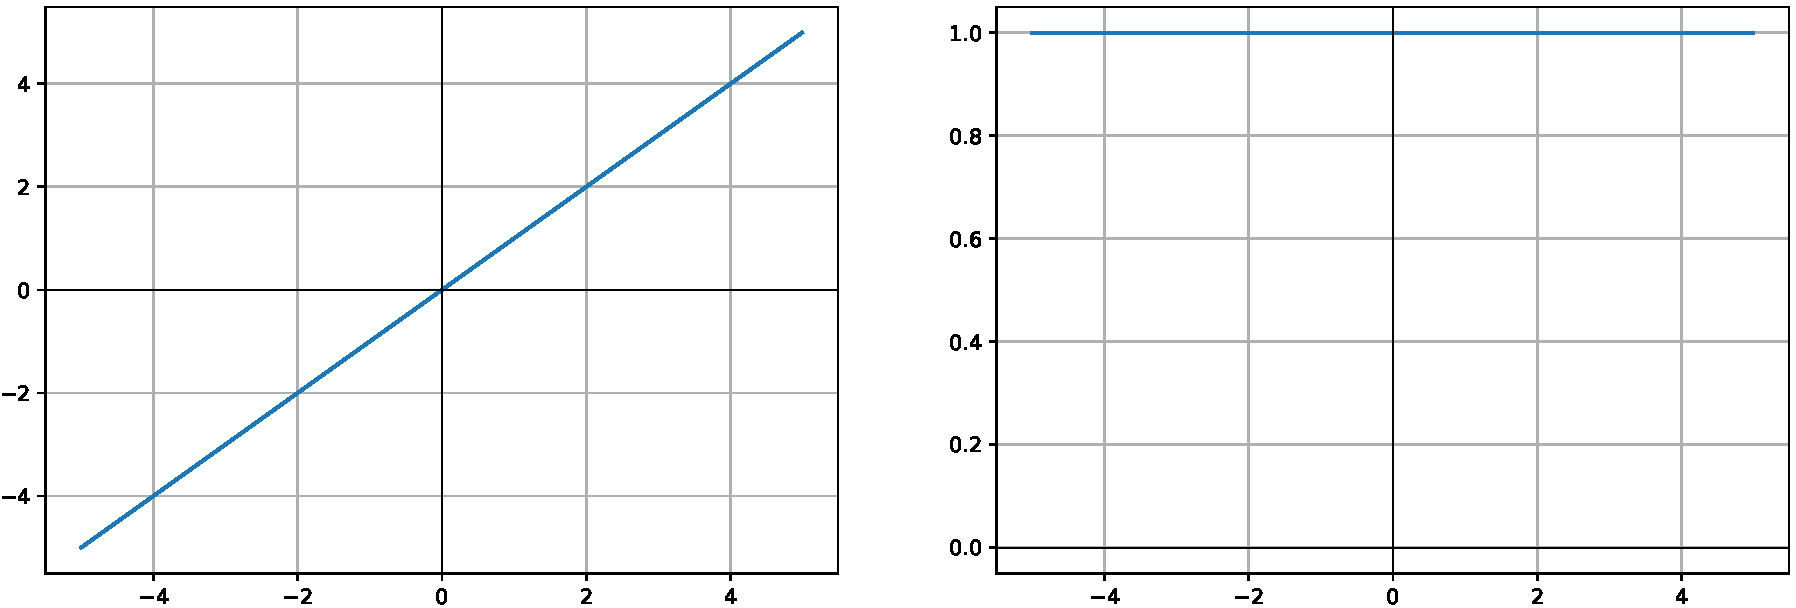
\includegraphics[width=\textwidth]{Identity.pdf}
\centering
\caption{Funkcija identiteta i njena derivacija}
\label{fig:identity}
\end{figure}

\begin{equation}
\begin{split}
f(x) = x
\end{split}
\qquad
\begin{split}
f'(x) = 1
\end{split}
\end{equation}

Funkcija identiteta je jednostavna i brza, no njome neuronska mreža može naučiti samo linearne funkcije. Ako primijenimo funkciju na dva uzastopna sloja vidimo da je konačna funkcija ponovno linearna što znači da ne možemo naučiti mrežu na nelinearnim podatcima:
\begin{align}
\begin{split}
f_l(x) &= w_l \cdot x + b_l \\
f_1(f_2(x)) &= w_1 \cdot (w_2 \cdot x + b_2) + b_1 \\
&= \underline{w_1 \cdot w_2} \cdot x + \underline{w_1 \cdot b_2 + b_1} \\
&= w_{1,2} \cdot x + b_{1,2}
\end{split}
\end{align}

\subsection{Zglobnica ili ispravljena linearna jedinica (ReLU)}
\label{func:relu}
\engl{Rectified linear unit}

\begin{figure}[H]
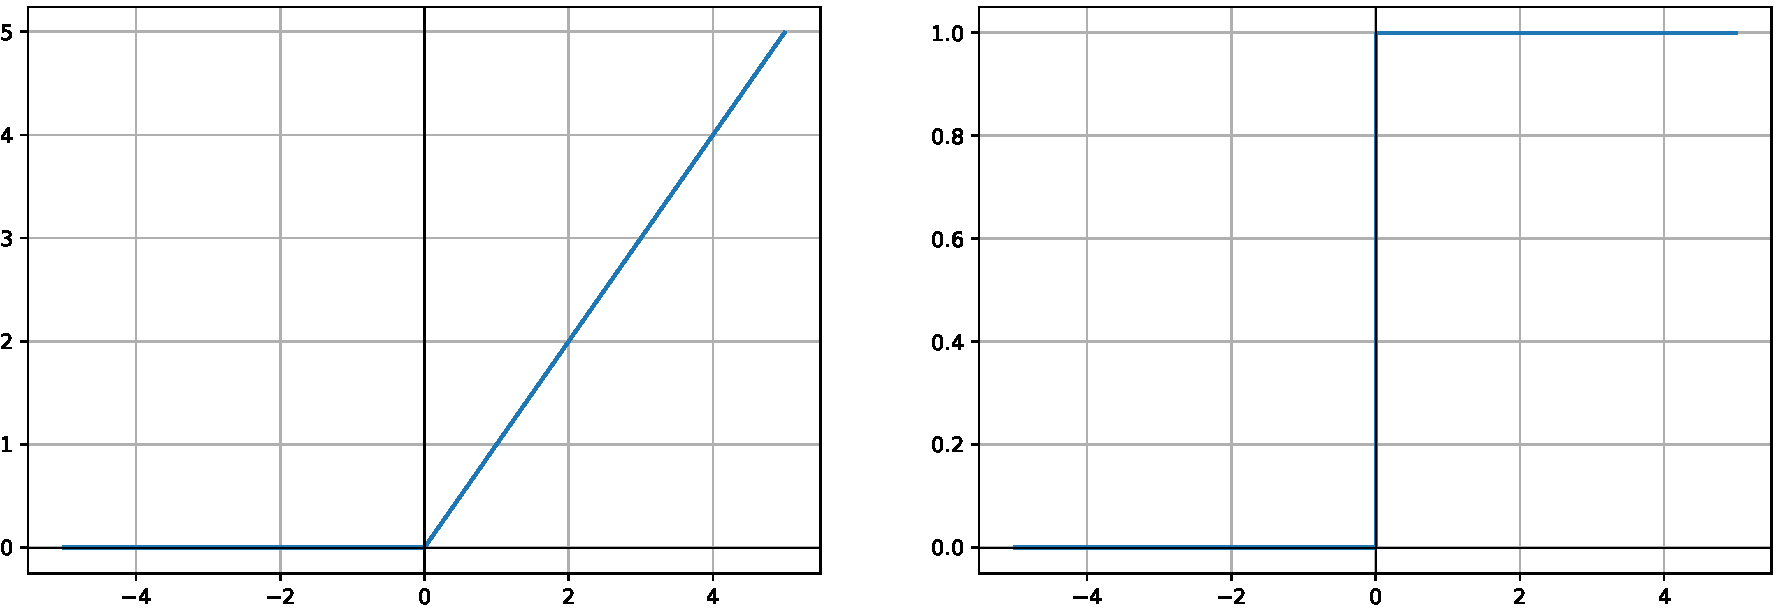
\includegraphics[width=\textwidth]{ReLU.pdf}
\centering
\caption{Funkcija ReLU i njena derivacija}
\label{fig:relu}
\end{figure}

\begin{equation}
\label{eq:relu}
\begin{split}
f(x) &= \begin{cases}
x,		& \text{ako } x > 0 \\
0,		& \otherwise
\end{cases} \\
&= max(0, x)
\end{split}
\qquad
\begin{split}
f'(x) = 
\begin{cases}
1,		& \text{ako } x > 0 \\
0,		& \otherwise
\end{cases}
\end{split}
\end{equation}

Funkcija ReLU svoje korijene povlači iz rada bioloških neurona, a u dubokom učenju je zamijenila dotadašnju sigmoidu i tangens hiperbolni. Zahvaljujući prizemljenosti na negativnoj domeni ReLU omogućava neuronskoj mreži učenje rijetke reprezentacije. Njihovim kombiniranjem u dubokoj mreži dobivamo model s eksponencijalno puno linearnih regija koje dijele zajedničke parametre \citep{relu_rbm}. Zahvaljujući linearnosti na pozitivnoj domeni funkcija ne doprinosi isčezavanju ni eksploziji gradijenta, a sam izračun funkcije i derivacije je vrlo brz i efikasan. \citep{relu}

Problem u negativnoj domeni je mogućnost blokiranja gradijenta i neaktivnih neurona (mrtvi neuroni), no dok god postoji put kroz mrežu gdje su neuroni aktivni (u pozitivnoj domeni) učenje će raditi, što pokazuju i rezultati \citep{relu}. Drugi problem je u neograničenosti funkcije u pozitivnoj domeni, no nju rješavamo regularizacijom koja ograničava veličinu ulaza u neuron \citep{relu}.

\subsection{Propusna ispravljena linearna jedinica (LReLU)}
\engl{Leaky ReLU}

\begin{figure}[H]
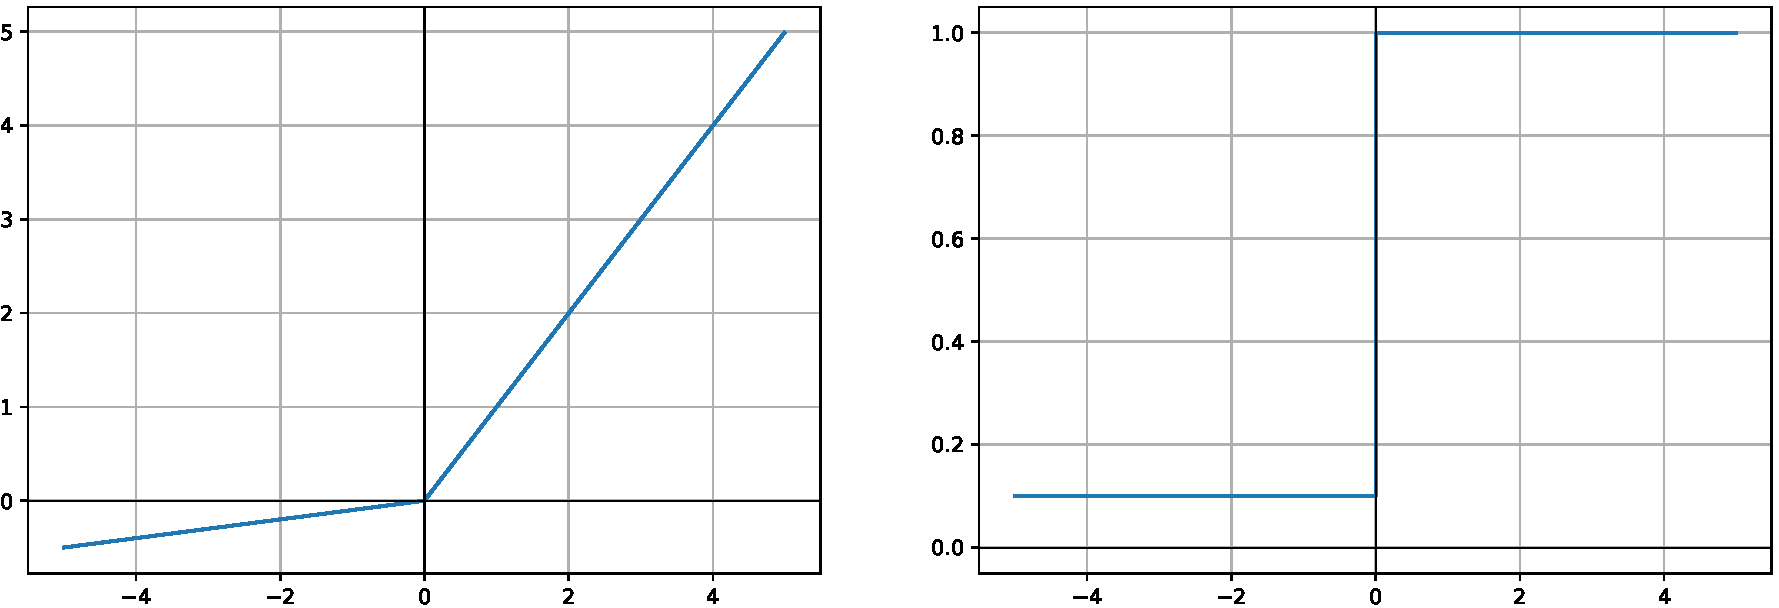
\includegraphics[width=\textwidth]{LReLU.pdf}
\centering
\caption{Funkcija LReLU i njena derivacija za $\alpha=0.1$}
\label{fig:lrelu}
\end{figure}

\begin{equation}
\begin{split}
f(x) &= \begin{cases}
x,			& \text{ako } x > 0 \\
\alpha x,	& \otherwise
\end{cases} \\
&= max(\alpha x, x)
\end{split}
\qquad
\begin{split}
f'(x) = 
\begin{cases}
1,		& \text{ako } x > 0 \\
\alpha,	& \otherwise
\end{cases}
\end{split}
\end{equation}

Problem funkcije ReLU \secref{func:relu} je što postoji mogućnost pojave mrtvih neurona, koji su uvijek u neaktivnom području i kroz njih ne teče gradijent. Taj problem efektivno smanjuje kapacitet modela pod cijenu nepotrebnog memorijskog opterećenja i smanjene brzine izvođenja. Iz navedenih razloga uvedena je propusna ReLU funkcija koja u "neaktivnom" području propušta mali gradijent. Rezultati na zadatku prepoznavanja govora pokazuju da je propusna ReLU funkcija ekvivalentna standardnom ReLU, no rezultati su prikazani na relativno plitkim arhitekturama (do 4 skrivena sloja). \citep{lrelu}

\subsection{Parametrizirana ispravljena linearna jedinica (PReLU)}
\engl{Parametric ReLU}

\todoimg{}


\begin{equation}
\begin{split}
f(x) &= \begin{cases}
x,			& \text{ako } x > 0 \\
\alpha x,	& \otherwise
\end{cases} \\
&= max(\alpha x, x)
\end{split}
\qquad
\begin{split}
f'(x) = 
\begin{cases}
1,		& \text{ako } x > 0 \\
\alpha,	& \otherwise
\end{cases}
\end{split}
\end{equation}
\begin{equation*}
\alpha \text{ je učeći parametar}
\end{equation*}

\todo{koji problem rješava}
\todo{svojstva}
\todo{problemi}

\subsection{Nasumična ispravljena linearna jedinica (RReLU)}
\engl{Randomized leaky ReLU}

\todoimg{}

\begin{equation}
\begin{split}
f(x) &= 
\begin{cases}
x,			& \text{ako } x > 0 \\
\alpha x,	& \otherwise
\end{cases}
\end{split}
\qquad
\begin{split}
f'(x) = 
\begin{cases}
1,		& \text{ako } x > 0 \\
\alpha,	& \otherwise
\end{cases}
\end{split}
\end{equation}
\begin{equation}
\alpha \sim U(l,u),\quad l,u \in [0,1]
\end{equation}

\todo{koji problem rješava}
\todo{svojstva}
\todo{problemi}

\subsection{Ispravljena linearna jedinica s pragom (ThReLU)}
\engl{Thresholded ReLU}

\begin{figure}[H]
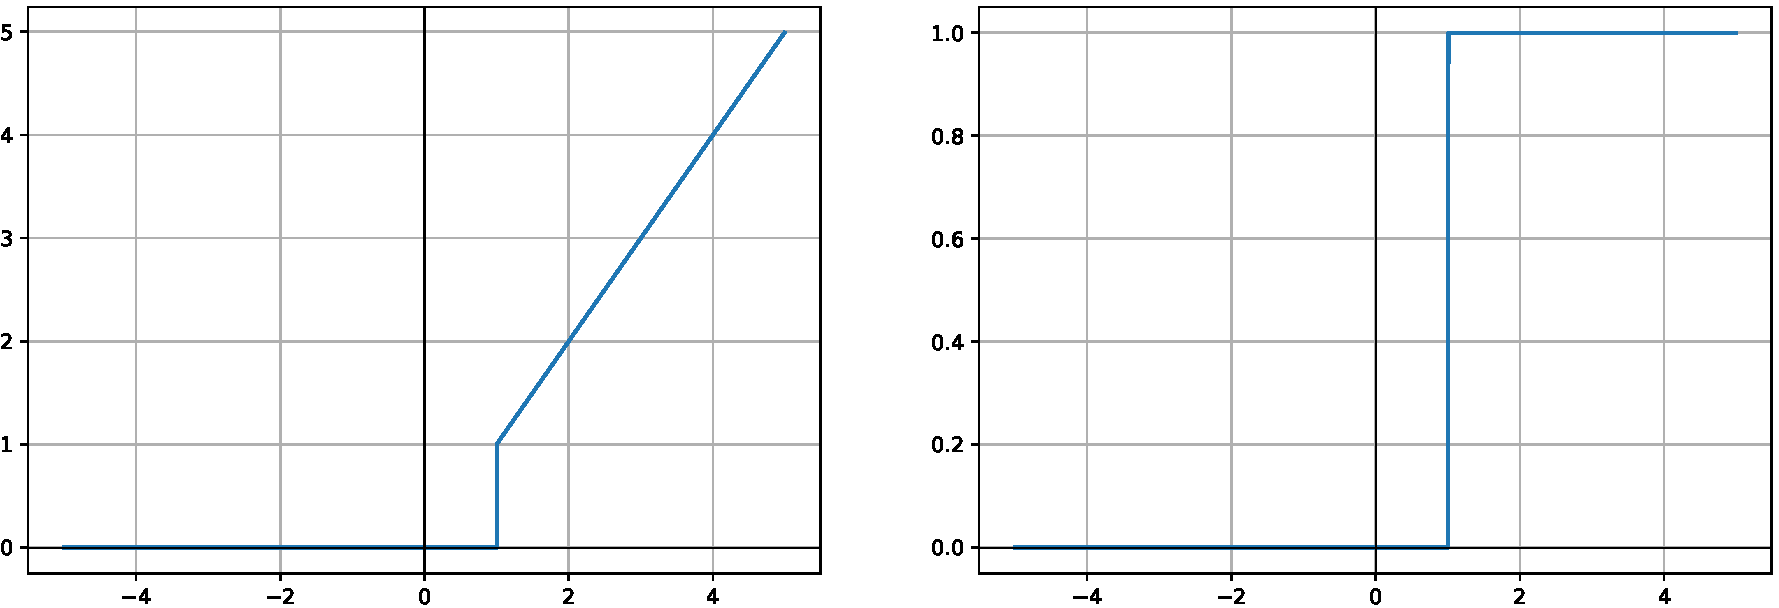
\includegraphics[width=\textwidth]{ThReLU.pdf}
\centering
\caption{Funkcija ThReLU i njena derivacija}
\label{fig:threlu}
\end{figure}

\begin{equation}
\begin{split}
f(x) = 
\begin{cases}
x,		& \text{ako } x > \theta \\
0,		& \otherwise
\end{cases}
\end{split}
\qquad
\begin{split}
f'(x) = 
\begin{cases}
1,		& \text{ako } x > \theta \\
0,		& \otherwise
\end{cases}
\end{split}
\end{equation}

\todo{koji problem rješava}
\todo{svojstva}
\todo{problemi}

\subsection{(CReLU)}
\engl{Concatenated ReLU}

\todoimg{}

\begin{equation}
???
\end{equation}

\todo{koji problem rješava}
\todo{svojstva}
\todo{problemi}

\subsection{Softplus}

\begin{figure}[H]
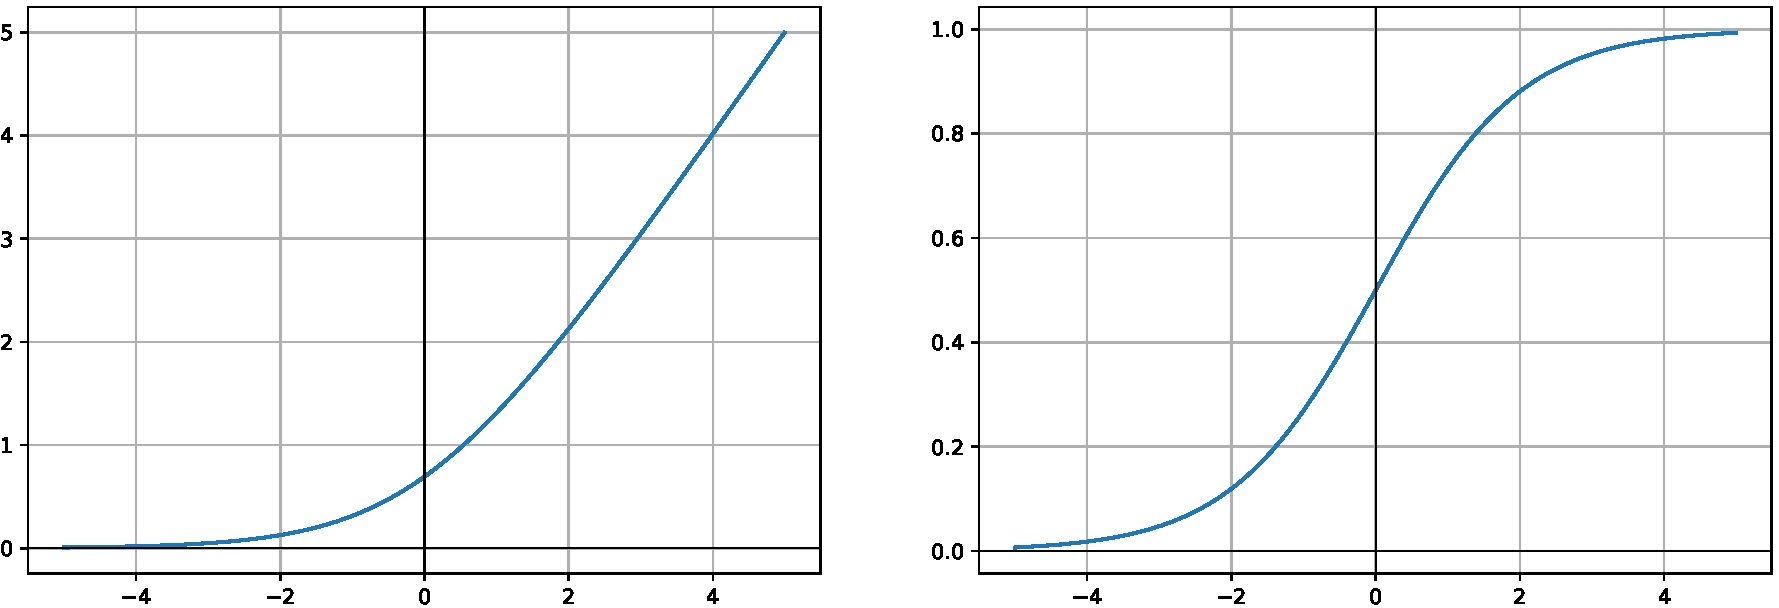
\includegraphics[width=\textwidth]{Softplus.pdf}
\centering
\caption{Softplus i njegova derivacija}
\label{fig:softplus}
\end{figure}

\begin{equation}
\begin{split}
f(x) = log(1+e^x)
\end{split}
\qquad
\begin{split}
f'(x) = \frac{e^x}{1+e^x}
\end{split}
\end{equation}

\todo{koji problem rješava}
\todo{svojstva}
\todo{problemi}

Funkcija Softplus nastaje ...

\subsection{Noisy softplus}

\todoimg{}

\begin{equation}
???
\end{equation}

\todo{koji problem rješava}
\todo{svojstva}
\todo{problemi}

\subsection{Eksponencijalno-linearna jedinica (ELU)}
\engl{Exponential linear unit}

\begin{figure}[H]
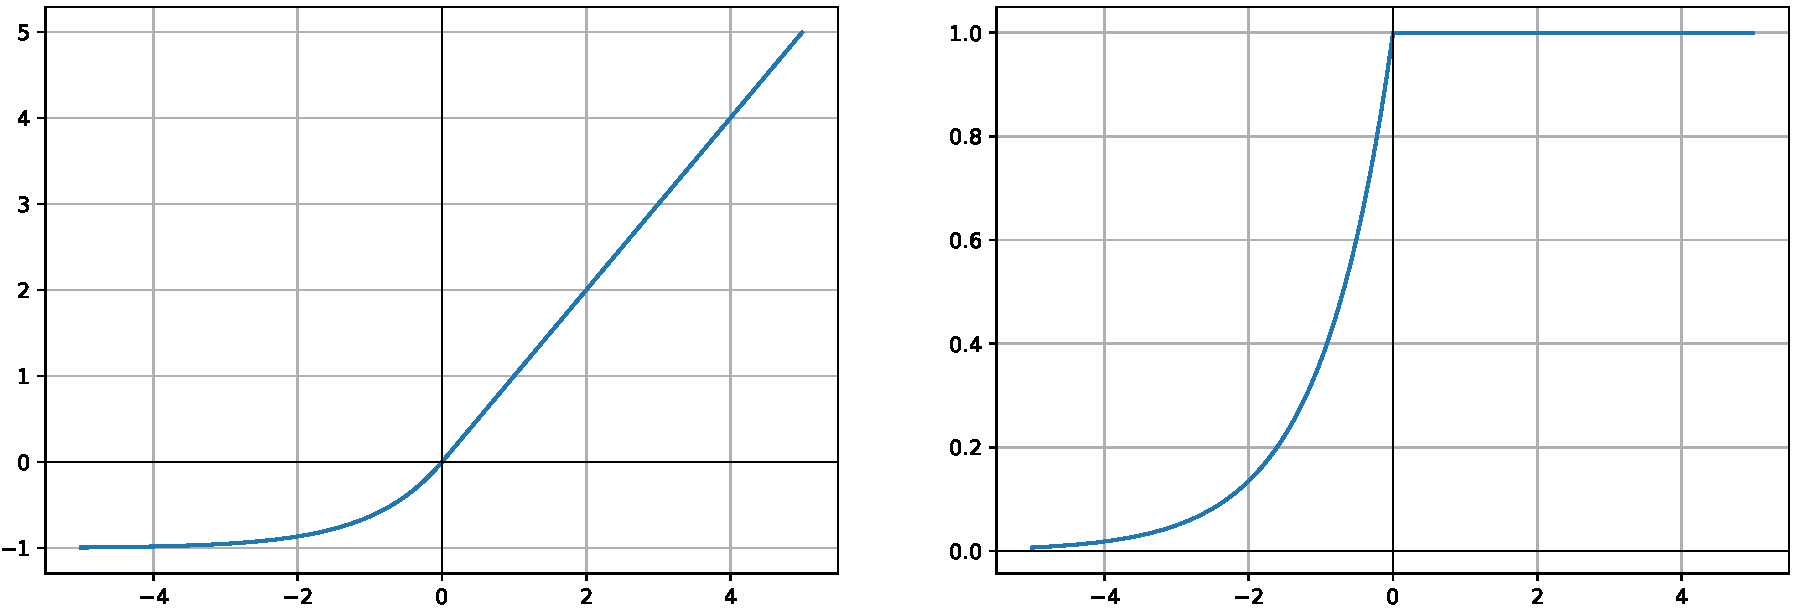
\includegraphics[width=\textwidth]{ELU.pdf}
\centering
\caption{Funkcija ELU i njena derivacija}
\label{fig:elu}
\end{figure}

\begin{equation}
\label{eq:elu}
\begin{split}
f(x) = 
\begin{cases}
x,					& \text{ako } x > 0 \\
\alpha (e^x - 1),	& \otherwise
\end{cases}
\end{split}
\qquad
\begin{split}
f'(x) = 
\begin{cases}
1,	 		& \text{ako } x > 0 \\
\alpha e^x,	& \otherwise
\end{cases}
\end{split}
\end{equation}

\todo{koji problem rješava}
\todo{svojstva}
\todo{problemi}

\subsection{Skalirana eksponencijalno-linearna jedinica (SELU)}
\engl{Scaled exponential linear unit}

\begin{figure}[H]
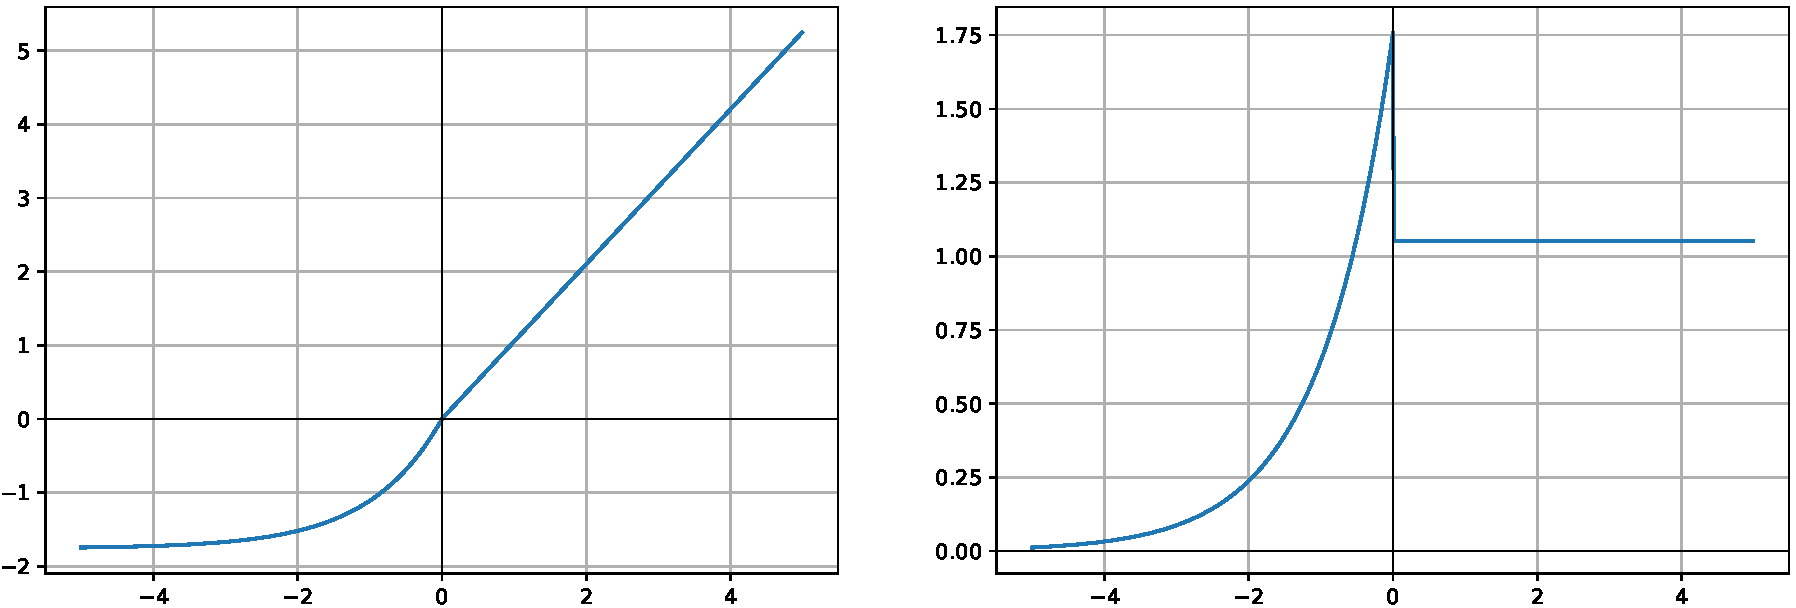
\includegraphics[width=\textwidth]{SELU.pdf}
\centering
\caption{Funkcija SELU i njena derivacija}
\label{fig:selu}
\end{figure}

\begin{equation}
\begin{split}
f(x) = \lambda
\begin{cases}
x,					& \text{ako } x > 0 \\
\alpha (e^x - 1),	& \otherwise
\end{cases}
\end{split}
\qquad
\begin{split}
f'(x) = \lambda
\begin{cases}
1,	 		& \text{ako } x > 0 \\
\alpha e^x,	& \otherwise
\end{cases}
\end{split}
\end{equation}

\todo{koji problem rješava}
\todo{svojstva}
\todo{problemi}

\subsection{(GELU)}
\engl{Gaussian error linear unit}

\todoimg{}

\todo{koji problem rješava}
\todo{svojstva}
\todo{problemi}

\subsection{Swish}
\label{func:swish}

\begin{figure}[H]
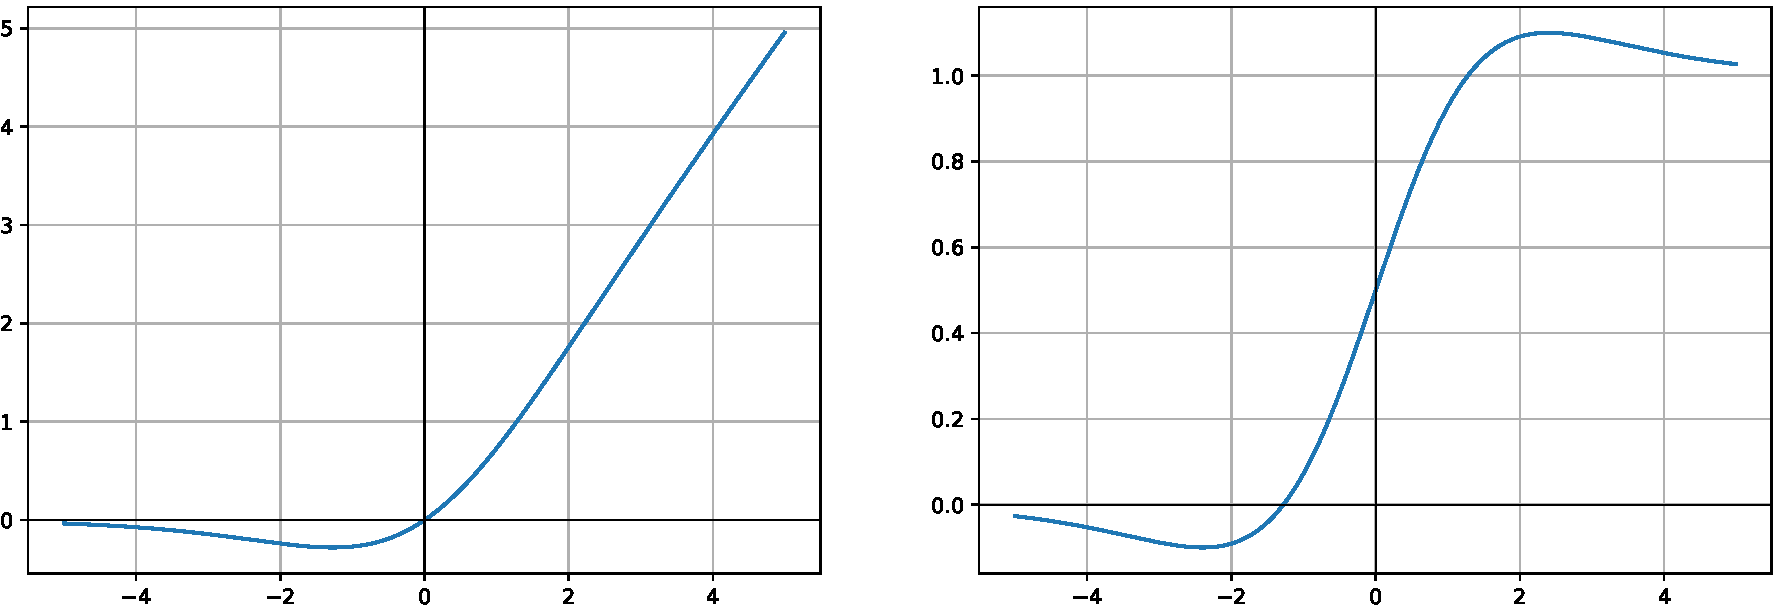
\includegraphics[width=\textwidth]{Swish.pdf}
\centering
\caption{Funkcija Swish i njena derivacija}
\label{fig:swish}
\end{figure}

\begin{equation}
\label{eq:swish}
\begin{split}
&f(x) = x \cdot \sigma(\beta x)
\\
&f'(x) = \sigma(\beta x) \cdot (1 + \beta x \cdot (1-\sigma(\beta x)) = \frac{e^x \cdot (e^x + x + 1)}{(e^x + 1)^2}
\end{split}
\end{equation}

\todo{koji problem rješava}
\todo{svojstva}
\todo{problemi}

\subsection{ELiSH}
\label{func:elish}
\engl{Exponential Linear Sigmoid Squashing}

\begin{figure}[H]
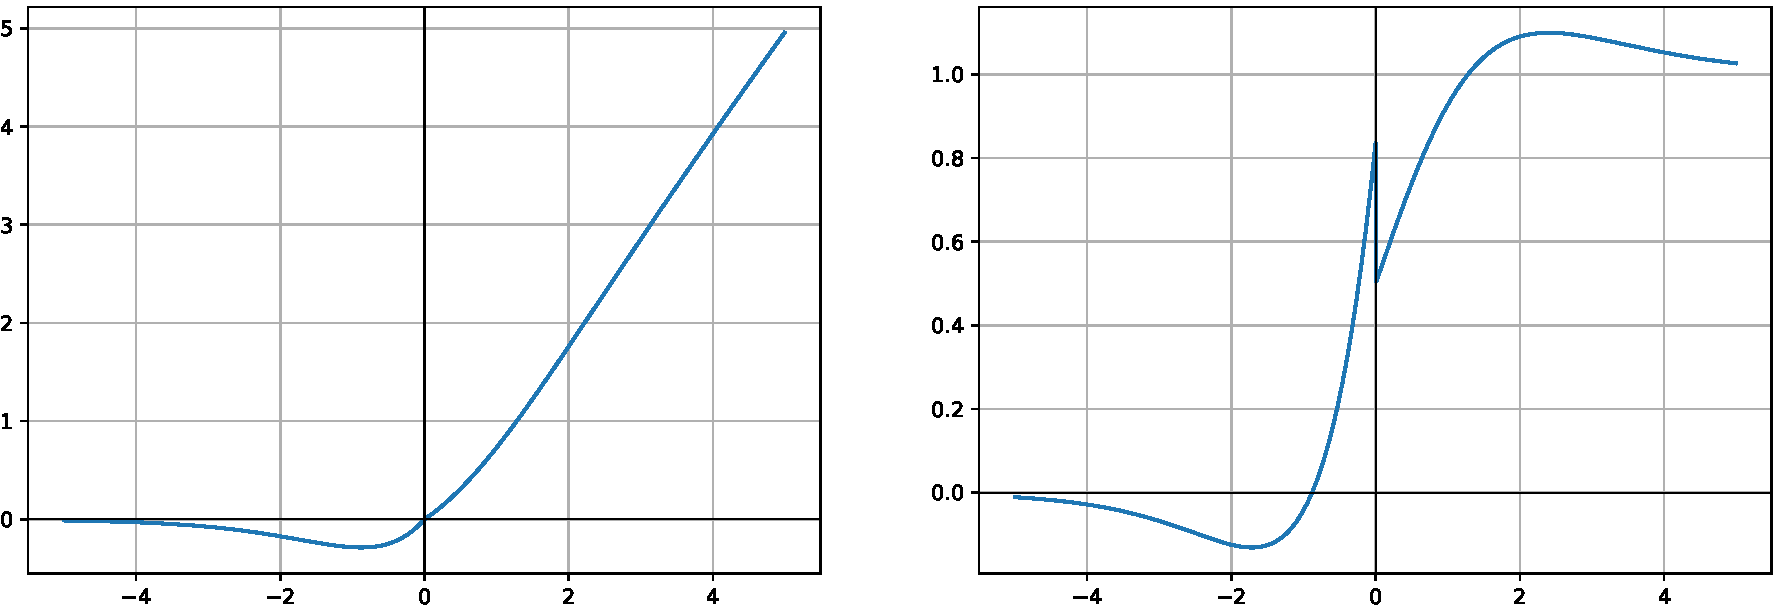
\includegraphics[width=\textwidth]{ELiSH.pdf}
\centering
\caption{Funkcija ELiSH i njena derivacija}
\label{fig:elish}
\end{figure}

\begin{equation}
\begin{split}
&f(x) = 
	\begin{cases}
		swish(x), \quad x \geq 0 \\
		ELU(x) \cdot \sigma(x), \quad \otherwise
	\end{cases} \\
&f'(x) =
	\begin{cases}
		swish'(x), \quad x \geq 0 \\
		\sigma(x) \cdot (ELU'(x) + ELU(x) \cdot (1-\sigma(x)), \quad \otherwise
	\end{cases}
\end{split}
\end{equation}

Ova funkcija i njena brža aproksimacija \textit{Tvrdi ELiSH} su kompozicije funkcija, različito definirane na pozitivnoj i negativnoj domeni. ELiSH pozitivnu domenu naslijeđuje od funkcije Swish \eqref{eq:swish}, a negativna je umnožak funkcije ELU \eqref{eq:elu} i sigmoide \eqref{eq:sigmoid}. Obje funkcije su ručno izgrađene s ciljem iskorištavanja dobrog prijenosa informacije koji ostvaruju funkcije Swish i sigmoida te sprečavanjem isčezavajućeg gradijenta pomoću linearne komponente u funkciji Swish. \citep{elish}

\subsection{Tvrdi ELiSH}
\label{func:hard_elish}
\engl{Hard ELiSH}

\begin{figure}[H]
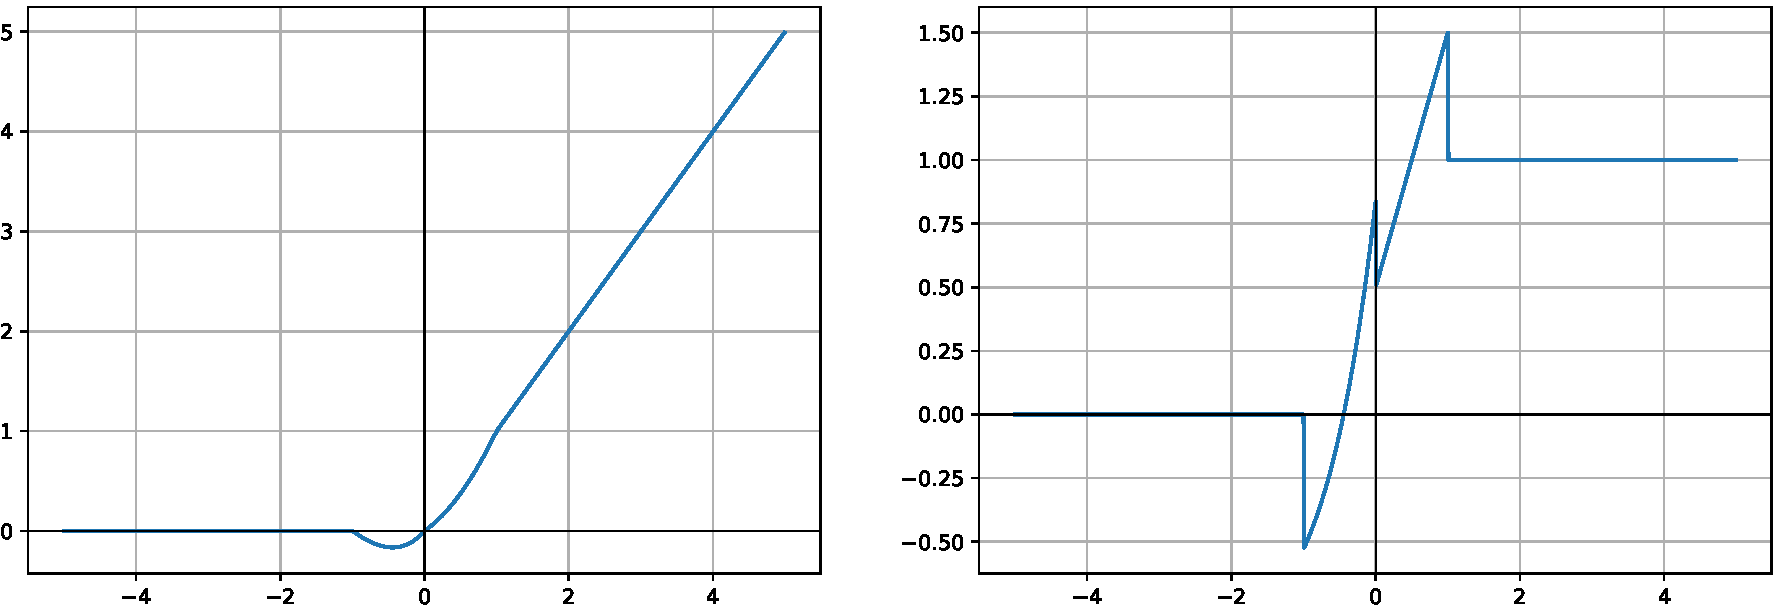
\includegraphics[width=\textwidth]{Hard_ELiSH.pdf}
\centering
\caption{Funkcija Tvrdi ELiSH i njena derivacija}
\label{fig:hard_elish}
\end{figure}

\begin{equation}
\begin{split}
&f(x) =
	\begin{cases}
		x \cdot a(x), \quad x \geq 0 \\
		ELU(x) \cdot a(x), \quad \otherwise
	\end{cases} \\
&f'(x) = \begin{cases}
	a(x) + x \cdot a'(x), \quad x \geq 0 \\
	ELU'(x) \cdot a(x) + x \cdot ELU(x) \cdot a'(x), \quad \otherwise
\end{cases}
\end{split}
\end{equation}

\begin{equation}
\begin{split}
&a(x) = \max(0, \min(1, \frac{x+1}{2})) \approx HardSigmoid(x) \\
&a'(x) =
\begin{cases}
	0.5, \quad |x| \leq 1 \\
	0, \quad \otherwise
\end{cases}	
\end{split}
\end{equation}

Ova funkcija je aproksimacija funkcije ELiSH opisane u poglavlju \ref{func:elish}. Uvedena je za potrebe bržeg izvođenja sigmoide i nasljeđuje svojstva ELiSH funkcije. \citep{elish}

\subsection{Ograničena ispravljena linearna jedinica (ReLUn)}
\label{func:relun}

\begin{figure}[H]
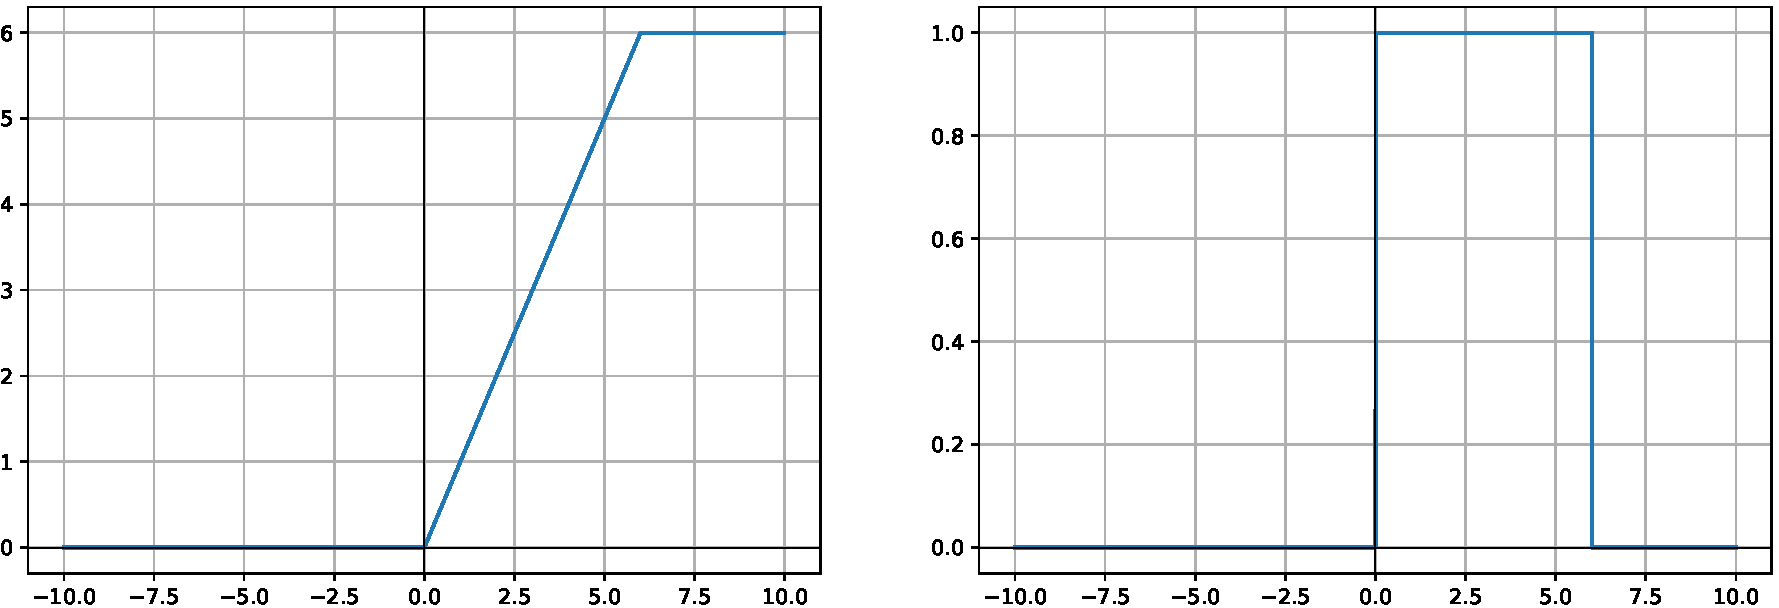
\includegraphics[width=\textwidth]{ReLU6.pdf}
\centering
\caption{Funkcija ReLU6 i njena derivacija}
\label{fig:relu6}
\end{figure}

\begin{equation}
\label{eq:relun}
\begin{split}
f(x) &= \begin{cases}
0,		& \text{ako } x < 0 \\
x,		& \text{ako } x \in [0, n] \\
n,		& \otherwise
\end{cases} \\
&= min(n, max(0, x))
\end{split}
\qquad
\begin{split}
f'(x) = 
\begin{cases}
1,		& \text{ako } x \in [0, n] \\
0,		& \otherwise
\end{cases}
\end{split}
\end{equation}
\begin{equation*}
n \in \realnum
\end{equation*}

Ograničena ReLU funkcija uvedena je kako bi ograničeni Boltzmann-ov stroj \engl{Restricted Boltzmann machine} brže naučio rijetke značajke, koje kasnije ugađa konvolucijski klasifikator. Za razliku od ReLU koji se može interpretirati kao kompozicija beskonačno mnogo identičnih Bernoullijevih jedinica translatiranih po domeni, ograničeni ReLU interpretiramo kao kompoziciju $n$ jedinica. Za vidljivi sloj korištena je ReLU1, a za skrivene slojeve ReLU6 funkcija. \citep{relu6}

S obzirom da je ReLUn neuron aktivan samo na relativno uskoj regiji u pozitivnoj domeni, postoji opasnost od pojave mrtvih neurona (kroz koje ne prolazi gradijent). Idealna regija je $<0,n>$ jer  je u njoj neuron aktivan, a učenjem se može specijalizirati približavanjem zasićenju i stvoriti rijetke reprezentacije. Stoga je potrebno koristiti regularizaciju te pažljivu inicijalizaciju parametara.

\subsection{Razlomljena linearna jedinica (PLU)}
\engl{Piecewise linear unit}

\begin{figure}[H]
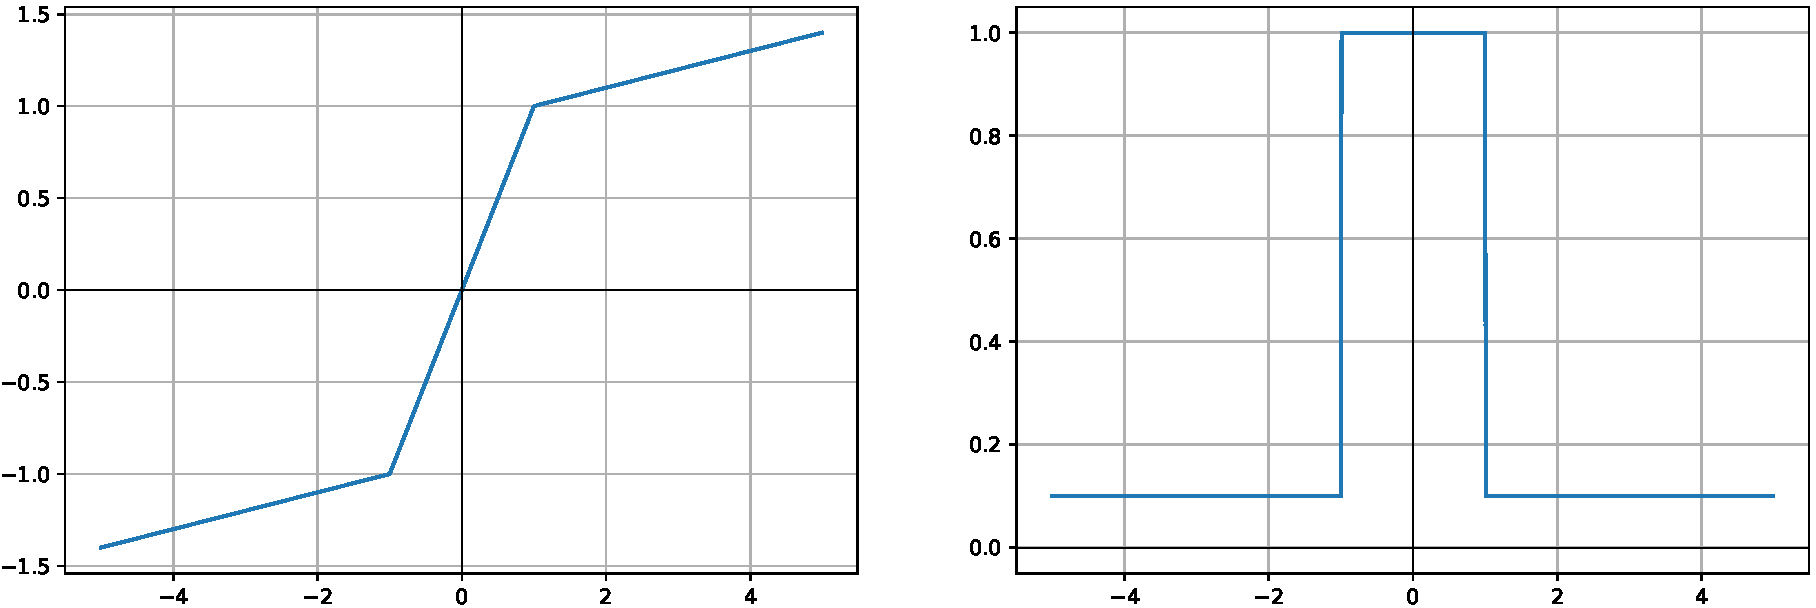
\includegraphics[width=\textwidth]{PLU.pdf}
\centering
\caption{Funkcija PLU i njena derivacija}
\label{fig:plu}
\end{figure}

\begin{equation}
\label{eq:plu}
\begin{split}
f(x) &=
\begin{cases}
x, \quad |x| \leq c \\
\alpha \cdot x, \quad \otherwise
\end{cases} \\
&= \max(\alpha x - c(1-\alpha), \min(x, \alpha x + c (1-\alpha)))
\end{split}
\quad
\begin{split}
f'(x) =
\begin{cases}
1, \quad |x| \leq c \\
\alpha, \quad \otherwise
\end{cases}
\end{split}
\end{equation}
\begin{equation*}
\alpha, c \in \realnum
\end{equation*}

\todo{koji problem rješava}
\todo{svojstva}
\todo{problemi}

\subsection{Sigmoida ($\sigma $)}
\engl{Sigmoid}

\begin{figure}[H]
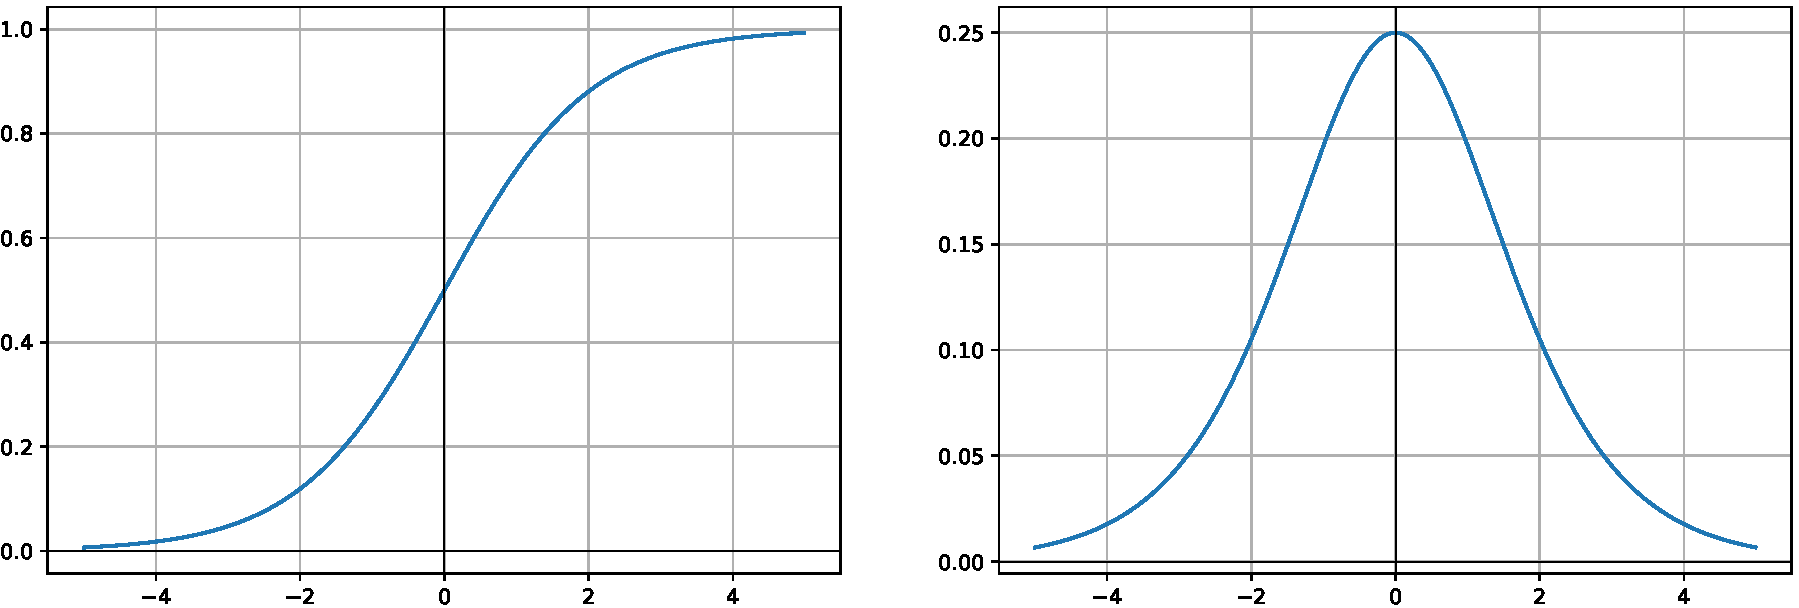
\includegraphics[width=\textwidth]{Sigmoid.pdf}
\centering
\caption{Sigmoida i njena derivacija}
\label{fig:sigmoid}
\end{figure}

\begin{equation}
\label{eq:sigmoid}
\begin{split}
f(x) = \frac{1}{1+e^{-x}}
\end{split}
\qquad
\begin{split}
f'(x) = \sigma(x)(1-\sigma(x))
\end{split}
\end{equation}

\todo{koji problem rješava}
\todo{svojstva}
\todo{problemi}

\subsection{Tvrda sigmoida}
\engl{Hard sigmoid}

\begin{figure}[H]
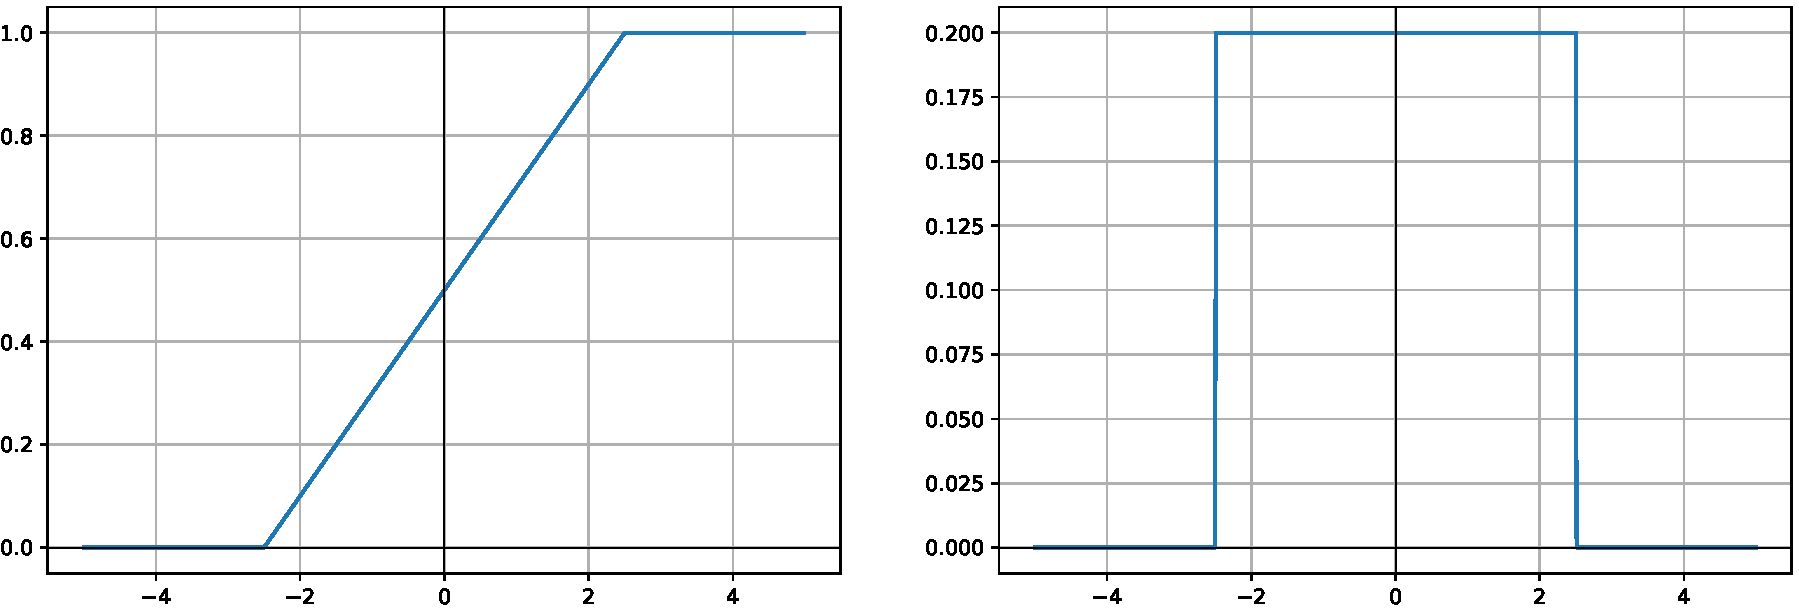
\includegraphics[width=\textwidth]{Hard_sigmoid.pdf}
\centering
\caption{Tvrda sigmoida i njena derivacija}
\label{fig:hard_sigmoid}
\end{figure}

\begin{equation}
\begin{split}
f(x) = min(1,\ max(0,\ 0.2x + 0.5))
\end{split}
\qquad
\begin{split}
f'(x) = 
\begin{cases}
0.2,	 		& \text{ako } |x| \leq 2.5 \\
0,	& \text{inače}
\end{cases}
\end{split}
\end{equation}

\todo{koji problem rješava}
\todo{svojstva}
\todo{problemi}

\subsection{Tangens hiperbolni (tanh)}
\label{func:tanh}

\begin{figure}[H]
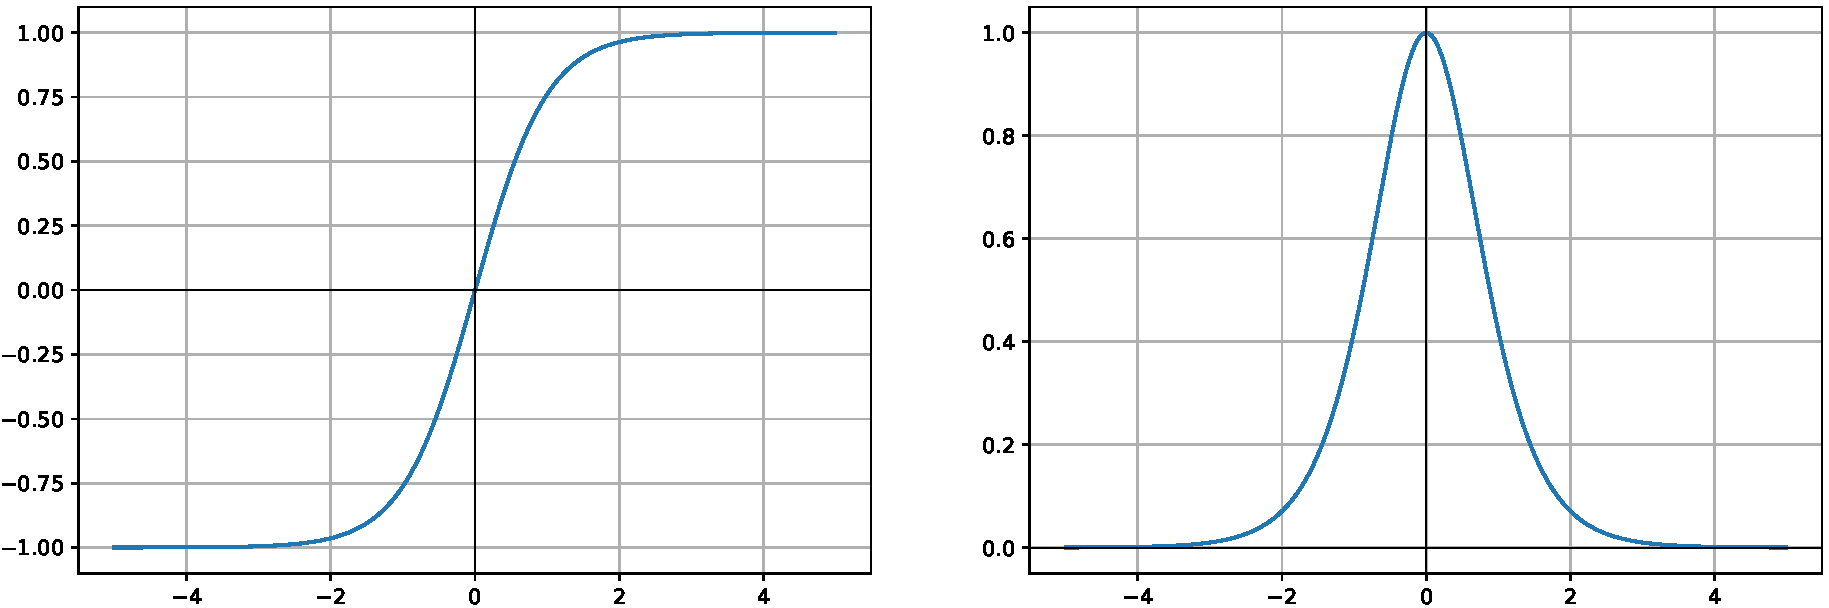
\includegraphics[width=\textwidth]{tanh.pdf}
\centering
\caption{Funkcija tanh i njena derivacija}
\label{fig:tanh}
\end{figure}

\begin{equation}
\begin{split}
f(x) = \frac{e^x - e^{-x}}{e^x + e^{-x}}
\end{split}
\qquad
\begin{split}
f'(x) = 1 - tanh^2(x)
\end{split}
\end{equation}

\todo{koji problem rješava}
\todo{svojstva}
\todo{problemi}

\subsection{Tvrdi tangens hiperbolni}
\engl{Hard tanh}

\begin{figure}[H]
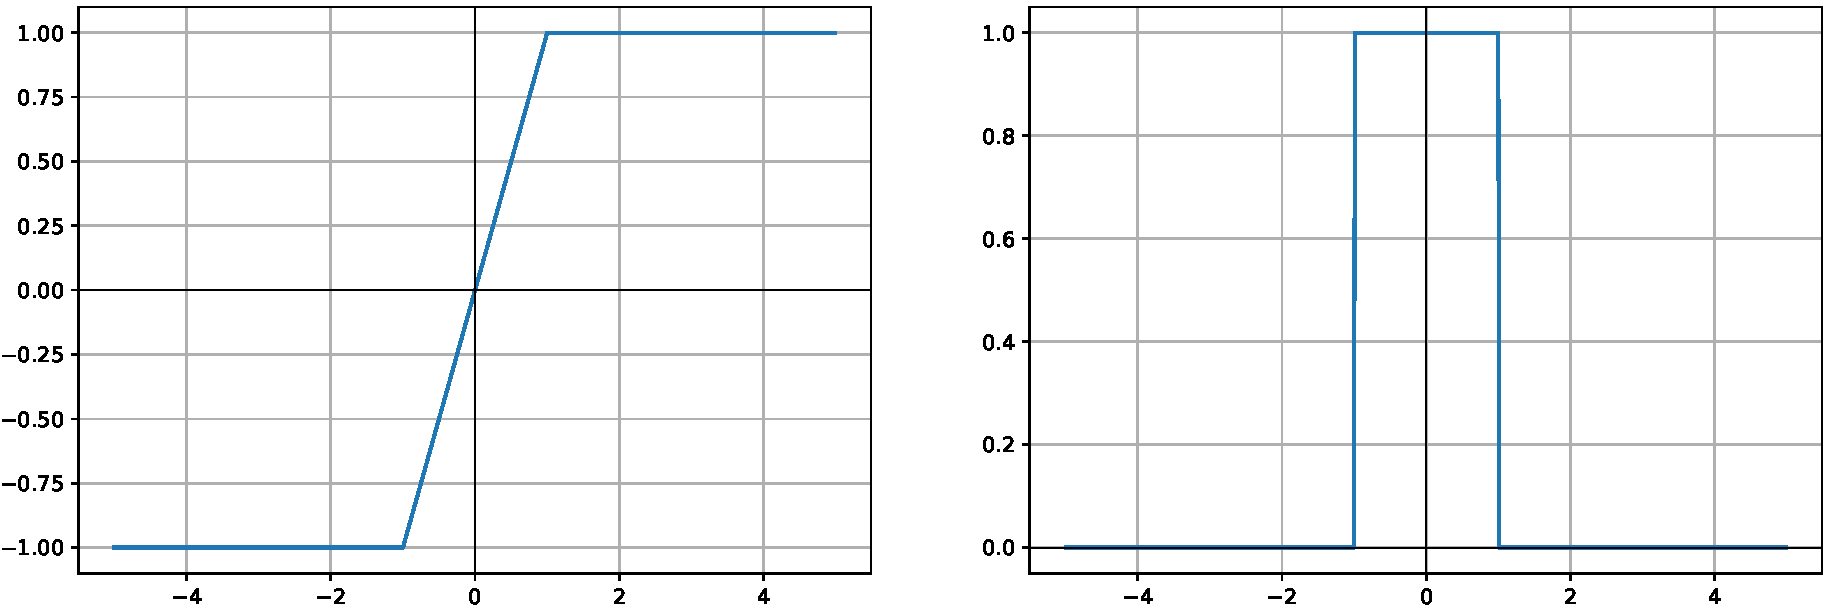
\includegraphics[width=\textwidth]{Hard_tanh.pdf}
\centering
\caption{Tvrdi tanh i njegova derivacija}
\label{fig:hard_tanh}
\end{figure}

\begin{equation}
\begin{split}
f(x) =
\begin{cases}
-1,	 		& \text{ako } x < 1 \\
x,	 		& \text{ako } |x| \leq 1 \\
1,	& \text{inače}
\end{cases}
\end{split}
\qquad
\begin{split}
f'(x) =
\begin{cases}
0,	 		& \text{ako } x < 1 \\
1,	 		& \text{ako } |x| \leq 1 \\
0,	& \text{inače}
\end{cases}
\end{split}
\end{equation}

\todo{koji problem rješava}
\todo{svojstva}
\todo{problemi}

\subsection{Racionalna aproksimacija tanh}
\engl{Rational tanh}

\begin{figure}[H]
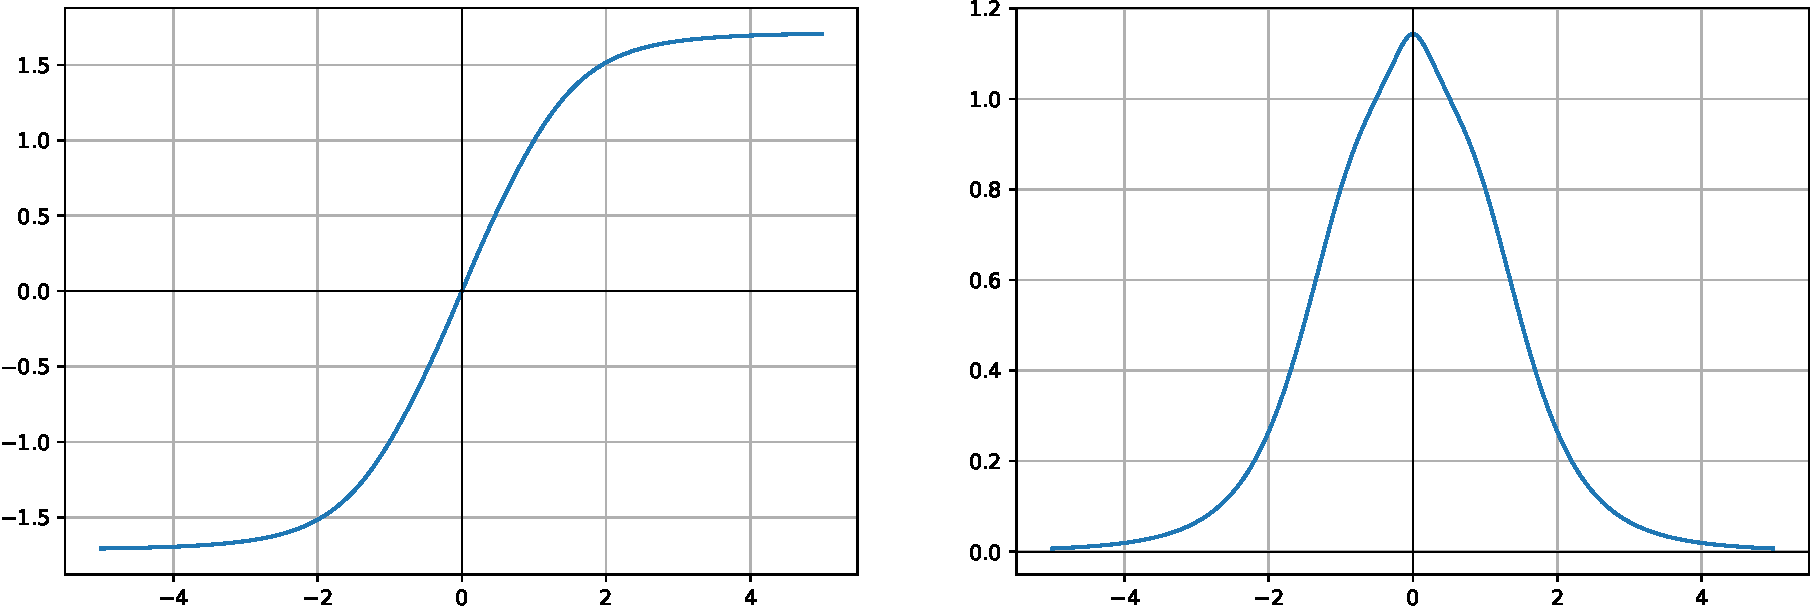
\includegraphics[width=\textwidth]{Rational_tanh.pdf}
\centering
\caption{Racionalni tanh i njegova derivacija}
\label{fig:rational_tanh}
\end{figure}

\begin{align}
\begin{split}
f(x) &= 1.7159 \cdot tanh^*(\frac{2}{3}x), \quad
tanh^*(x) = sgn(x)(1 - \frac{1}{1 + |x| + x^2 + 1.41645 \cdot x^4}) \\
f'(x) &= 1.7159 \cdot \frac{2}{3} \cdot tanh^{*'}(\frac{2}{3}x), \quad
tanh^{*'}(x) = \frac{1+sgn(x) \cdot (2x + 4 \cdot 1.41645 \cdot x^3)}{(1 + |x| + x^2 + 1.41645 \cdot x^4)^2}
\end{split}
\end{align}

\todo{koji problem rješava}
\todo{svojstva}
\todo{problemi}

\subsection{Ispravljeni tanh}
\engl{Rectified tanh}

\begin{figure}[H]
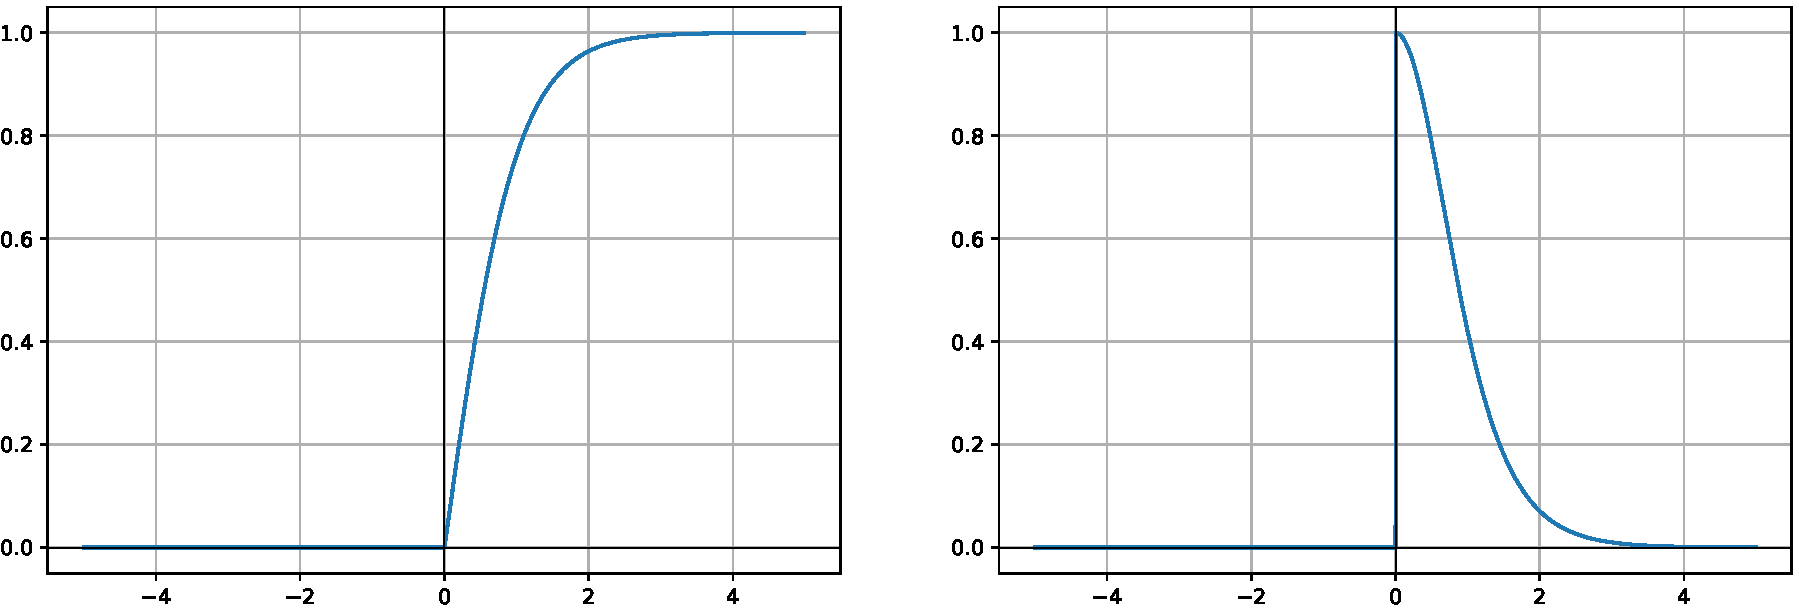
\includegraphics[width=\textwidth]{Rectified_tanh.pdf}
\centering
\caption{Ispravljeni tanh i njegova derivacija}
\label{fig:rectified_tanh}
\end{figure}

\begin{equation}
???
\end{equation}

\todo{koji problem rješava}
\todo{svojstva}
\todo{problemi}

\subsection{Softmax}

\todoimg{}

\begin{equation}
\begin{split}
f(\vec{x}) = \frac{e^{\vec{x}}}{\sum_ie^{\vec{x_i}}}
\end{split}
\qquad
\begin{split}
f'(x) = \frac{e^x}{1+e^x}
\end{split}
\end{equation}

\todo{koji problem rješava}
\todo{svojstva}
\todo{problemi}

\subsection{Hierarchical softmax}

\todoimg{}

\begin{equation}
???
\end{equation}

\todo{koji problem rješava}
\todo{svojstva}
\todo{problemi}


\subsection{Maxout}

\todoimg{}

\begin{equation}
???
\end{equation}

\todo{koji problem rješava}
\todo{svojstva}
\todo{problemi}

\subsection{Softsign}

\begin{figure}[H]
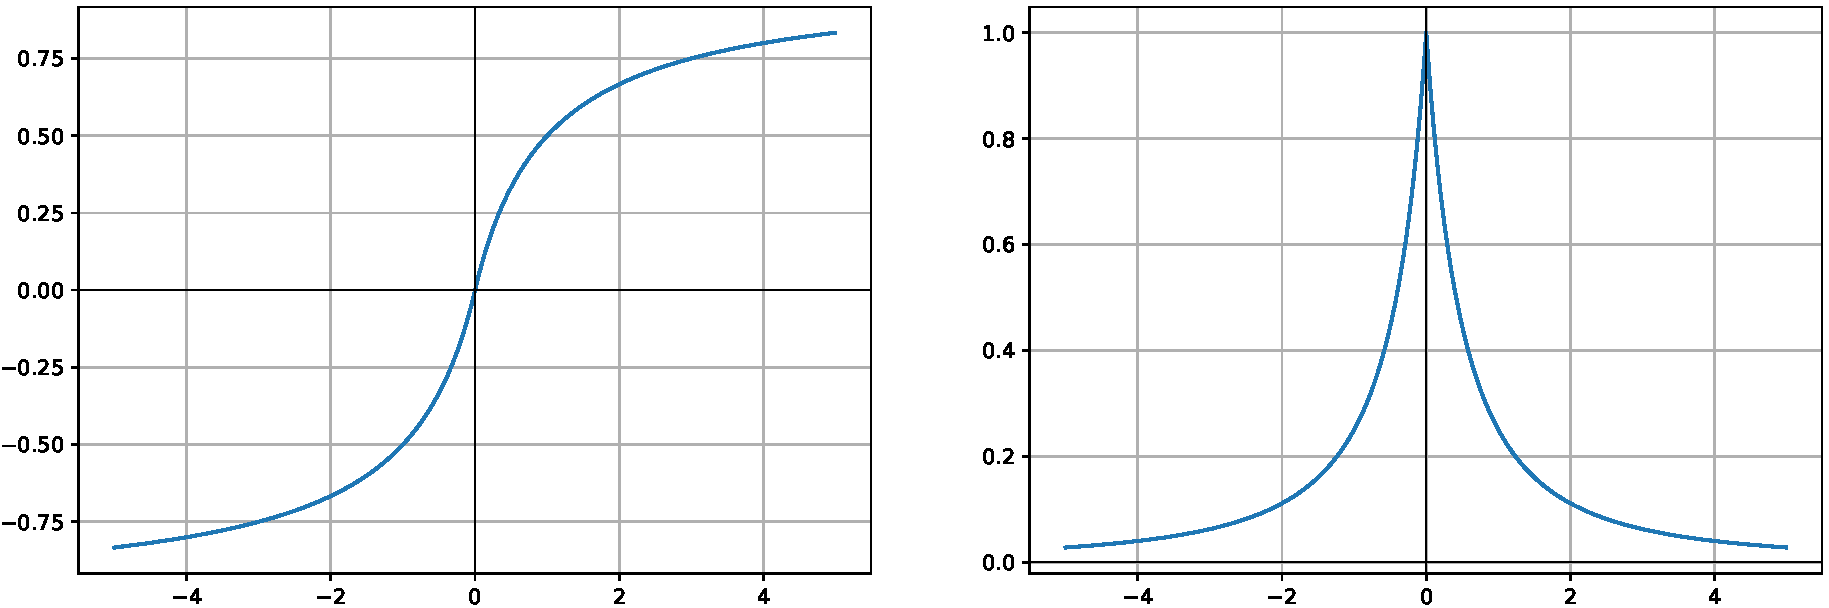
\includegraphics[width=\textwidth]{Softsign.pdf}
\centering
\caption{Softsign i njegova derivacija}
\label{fig:softsign}
\end{figure}

\begin{equation}
\begin{split}
f(x) = \frac{x}{1+|x|}
\end{split}
\qquad
\begin{split}
f'(x) = \frac{1 + |x| - x \cdot sign(x)}{(1+|x|)^2}
\end{split}
\end{equation}

\todo{koji problem rješava}
\todo{svojstva}
\todo{problemi}

\subsection{Sinus (sin)}

\begin{figure}[H]
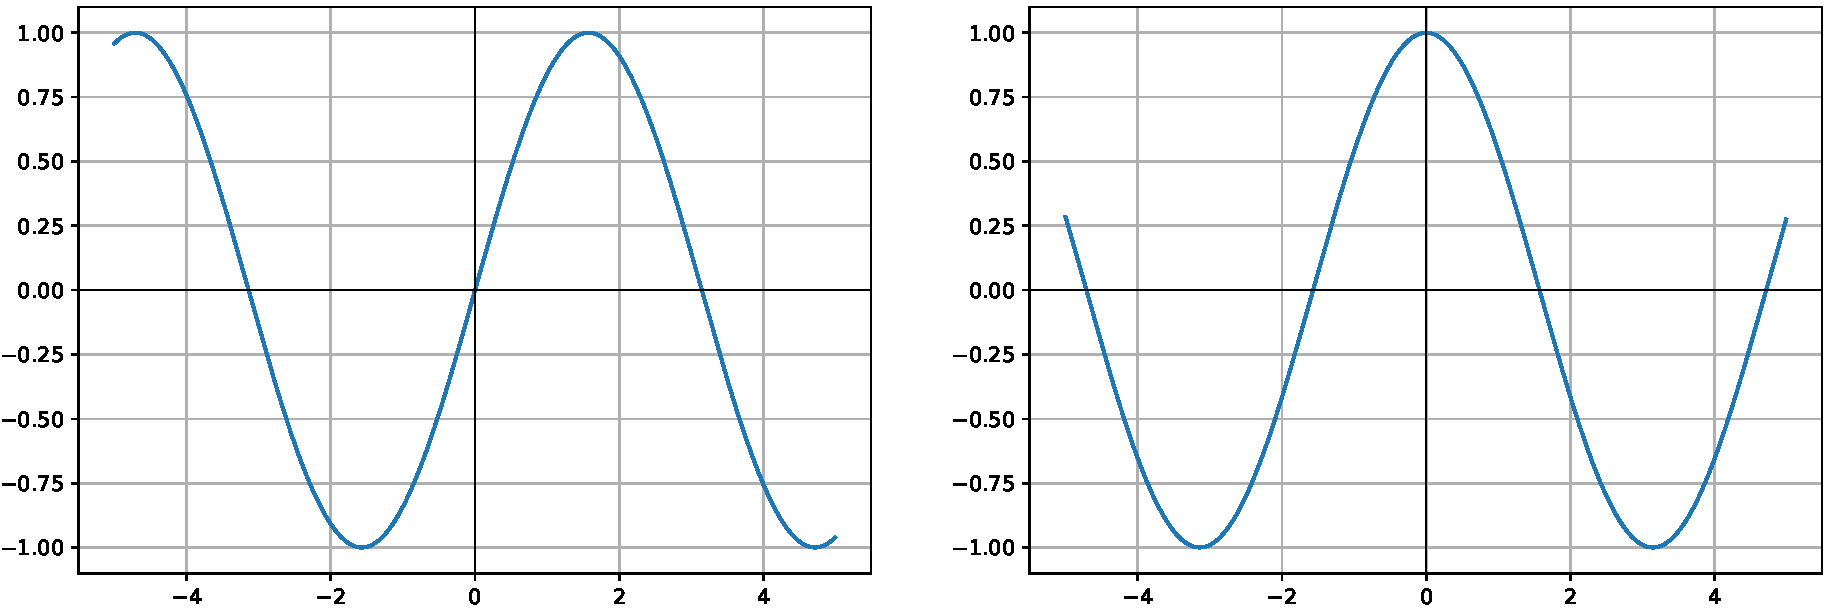
\includegraphics[width=\textwidth]{Sin.pdf}
\centering
\caption{Sinusoida i njegova derivacija}
\label{fig:sin}
\end{figure}

\begin{equation}
\begin{split}
f(x) = sin(x)
\end{split}
\qquad
\begin{split}
f'(x) = cos(x)
\end{split}
\end{equation}

Sinus je periodička funkcija te nema teorijsku podlogu za uporabu u neuronskim mrežama, za razliku od monotonih funkcija.
\todo{članak dokaz univerzalne aproksimacije monotonih fja}

Unatoč tome, pojavljuje se u radovima pretrage izlaznih funkcija \citep{elish} i u ovom radu te pokazuje obećavajuće rezultate. U radu \citet{taming_waves} autori predstavljaju problematiku učenja sa sinusoidom na jednostavnom problemu. Problem stvaraju brojni lokalni optimumi na koje je izrazito osjetljiv gradijentni spust. Problem je ublažava učenje stohastičkim gradijentnim spustom koji zaglađuje valovitost funkcije gubitka. Dodatno, autori pokazuju da neuronska mreža zapravo ne ovisi snažno o periodičnosti funkcije tako da su rezultate usporedili sa skraćenom sinusoidom \eqref{eq:truncated_sin}. Članak nije prošao postupak recenzije jer su dodatni eksperimenti urodili nekonzistentnim rezultatima u usporedbi s tangensom hiperbolnim.

Po uzoru na slićne funkcije kao što je sigmoida \figref{fig:sigmoid} i tangens hiperbolni \figref{fig:tanh}, sinusoida najveću vrijednost gradijenta daje upravo kada je aktivacija jednaka 0 (u ograničenom intervalu).

\subsection{Ograničeni sinus (TrSin)}
\label{func:trsin}
\engl{Truncated sine}

\begin{figure}[H]
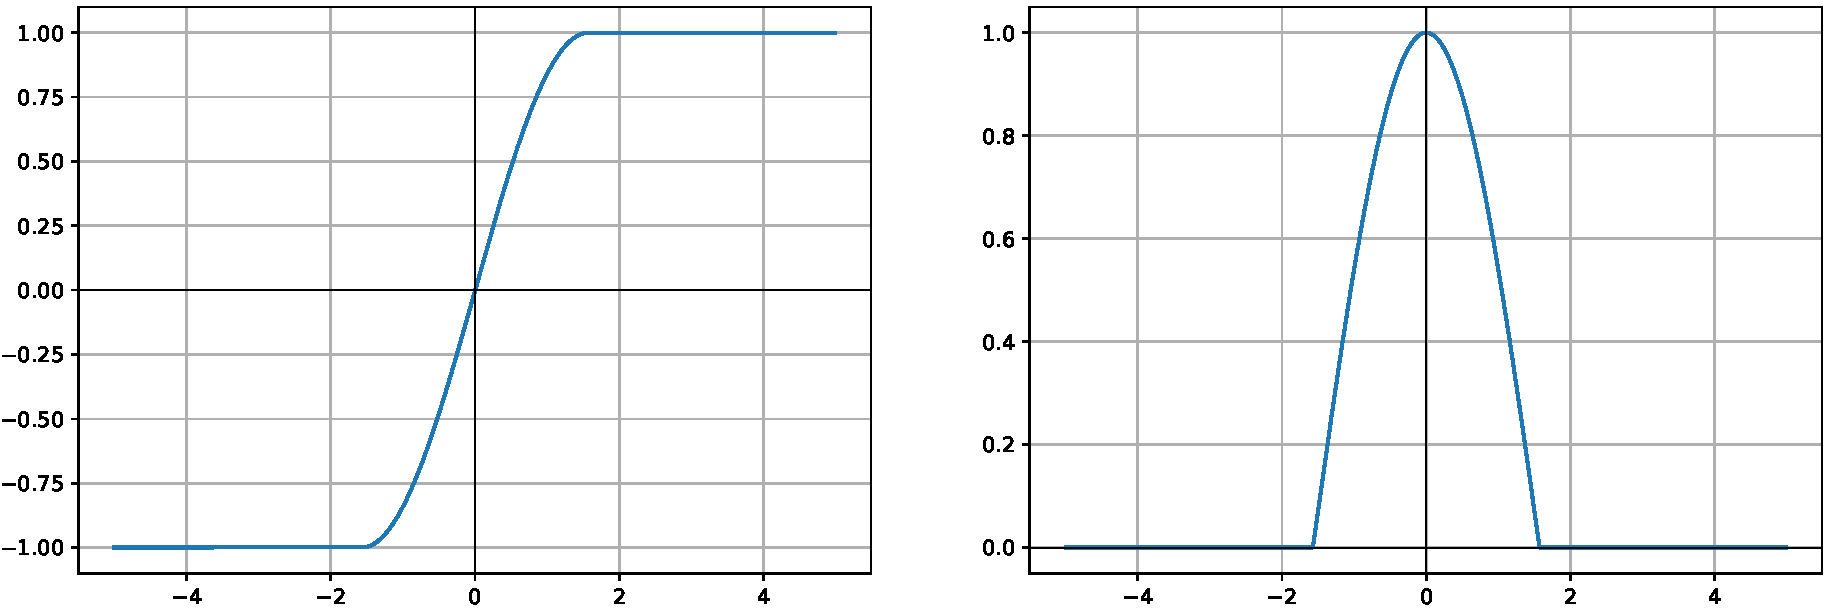
\includegraphics[width=\textwidth]{TrSin.pdf}
\centering
\caption{Ograničeni sinus i njegova derivacija}
\label{fig:trsin}
\end{figure}

\begin{equation}
\label{eq:trsin}
\begin{split}
f(x) =
\begin{cases}
0, \quad x < \frac{\pi}{2} \\
sin(x), \quad |x| \leq \frac{\pi}{2} \\
1, \quad \otherwise
\end{cases}
\end{split}
\qquad
\begin{split}
f'(x) =
\begin{cases}
cos(x), \quad |x| \leq \frac{\pi}{2} \\
0, \quad \otherwise
\end{cases}
\end{split}
\end{equation}

Ograničeni sinus korišten je u radu \citet{taming_waves} za usporedbu s klasičnom sinusoidom i tangensom hiperbolnim. U usporedbi sa sinusom ispituje se utjecaj periodičnosti sinusa na performanse. S tangensom hiperbolnim uspoređene su performanse zbog slićnosti u obliku krivulja.

\subsection{Kosinus (cos)}

\begin{figure}[H]
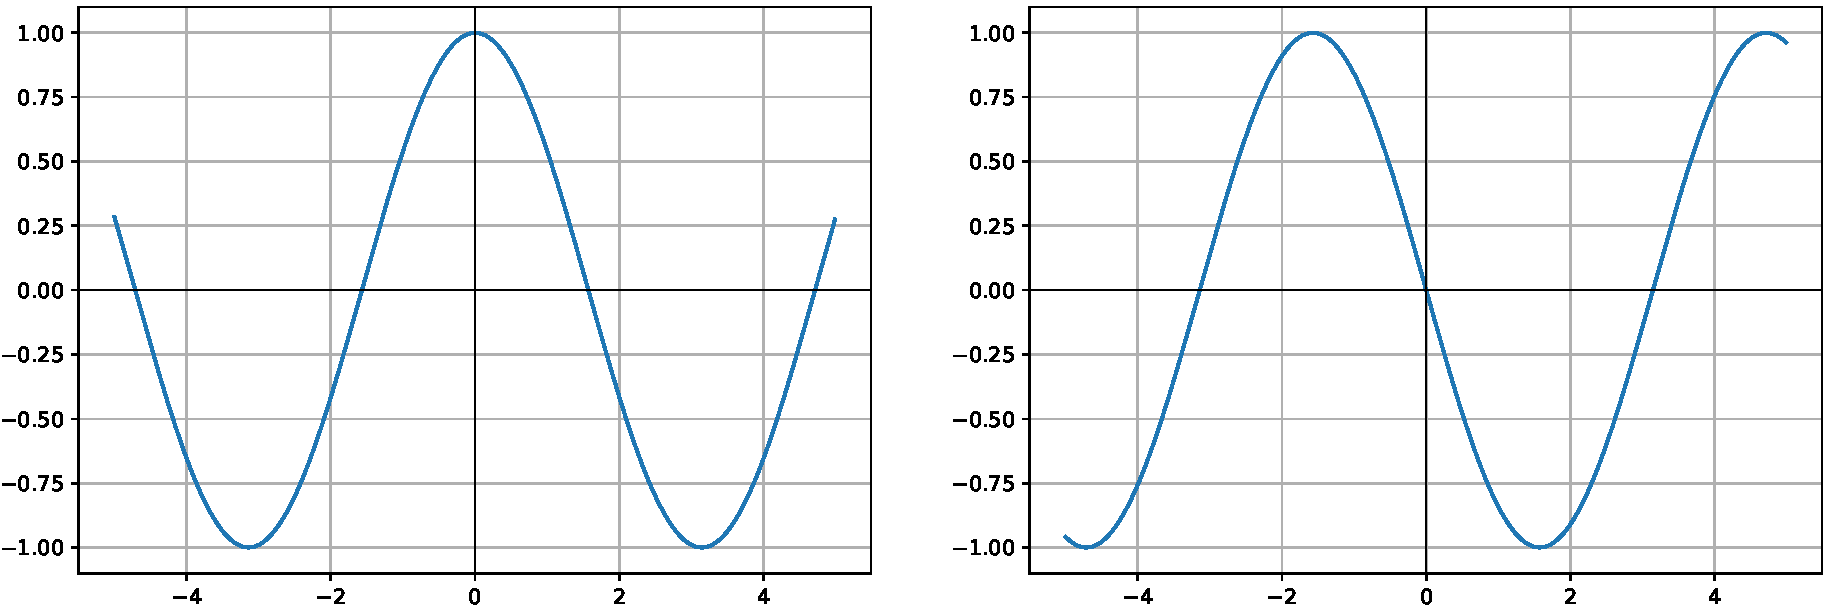
\includegraphics[width=\textwidth]{Cos.pdf}
\centering
\caption{Kosinus i njegova derivacija}
\label{fig:cos}
\end{figure}

\begin{equation}
\begin{split}
f(x) = cos(x)
\end{split}
\qquad
\begin{split}
f'(x) = -sin(x)
\end{split}
\end{equation}

Kosinus je funkcija sinusa pomaknuta za četvrtinu periode te dijeli ista svojstva i probleme. no, s obzirom da je pomak relativno velik u odnosu na očekivane veličine ulaza, možemo ga promatrati kao zasebnu izlaznu funkciju. Derivacija kosinusa se poprilično razlikuje od ostalih aktivacijskih funkcija. Unatoč tome, daje vrlo kompetitivne rezultate (poglavlje \ref{sec:rezultati}).
\begin{equation}
cos(x) = sin(x + \frac{\pi}{2}) \approx sin(x + 1.571)
\end{equation}

\subsection{Ograničeni kosinus (TrCos)}
\label{func:trcos}
\engl{Truncated cosine}

\begin{figure}[H]
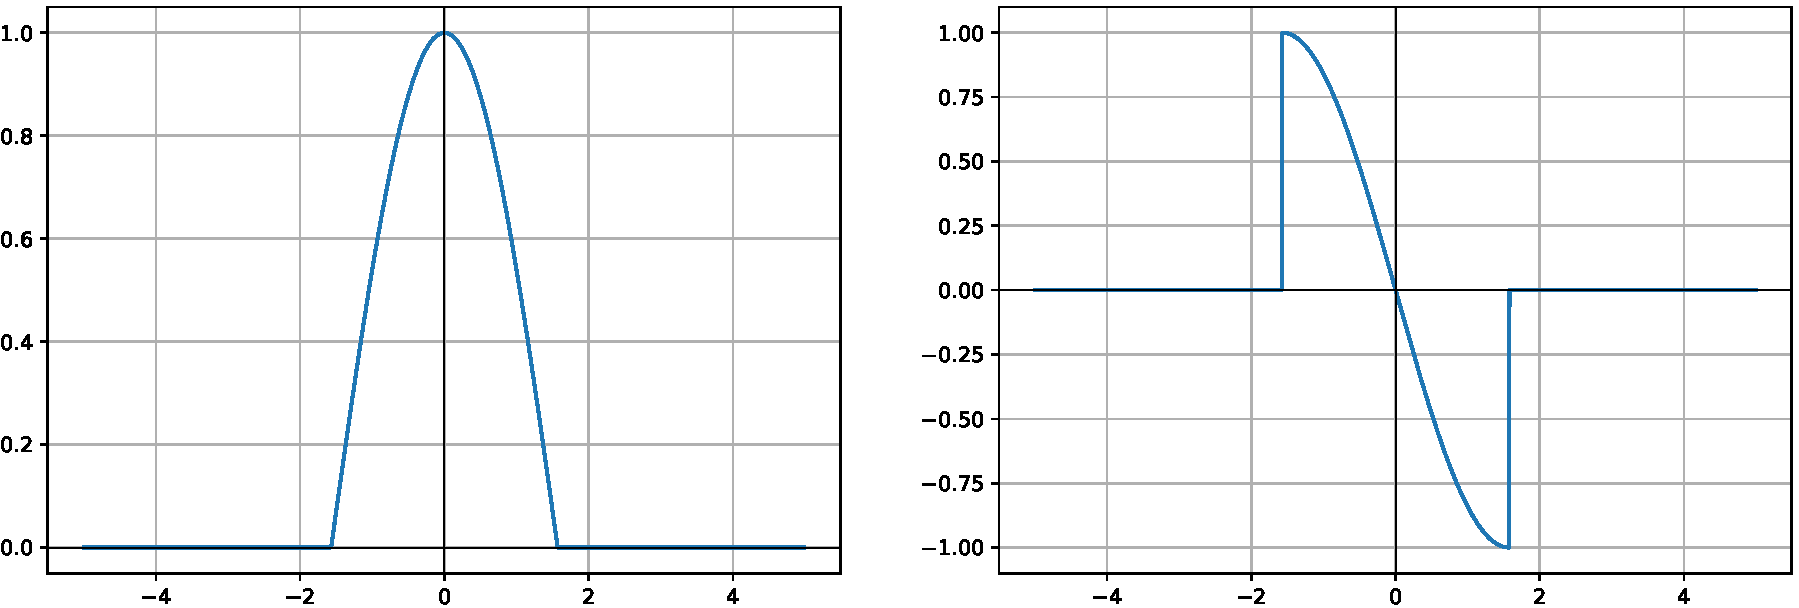
\includegraphics[width=\textwidth]{TrCos.pdf}
\centering
\caption{Ograničeni kosinus i njegova derivacija}
\label{fig:trcos}
\end{figure}

\begin{equation}
\label{eq:trcos}
\begin{split}
f(x) =
\begin{cases}
cos(x), \quad |x| \leq \frac{\pi}{2} \\
0, \quad \otherwise
\end{cases}
\end{split}
\qquad
\begin{split}
f'(x) =
\begin{cases}
-sin(x), \quad |x| \leq \frac{\pi}{2} \\
0, \quad \otherwise
\end{cases}
\end{split}
\end{equation}

Ograničeni kosinus autori nisu pronašli u literaturi, no navodi se zbog potrebe ispitivanja ovisnosti o periodičnosti kosinusa (po uzoru na poglavlje \ref{func:trsin}).

\subsection{Parabola $x^2$}

\begin{figure}[H]
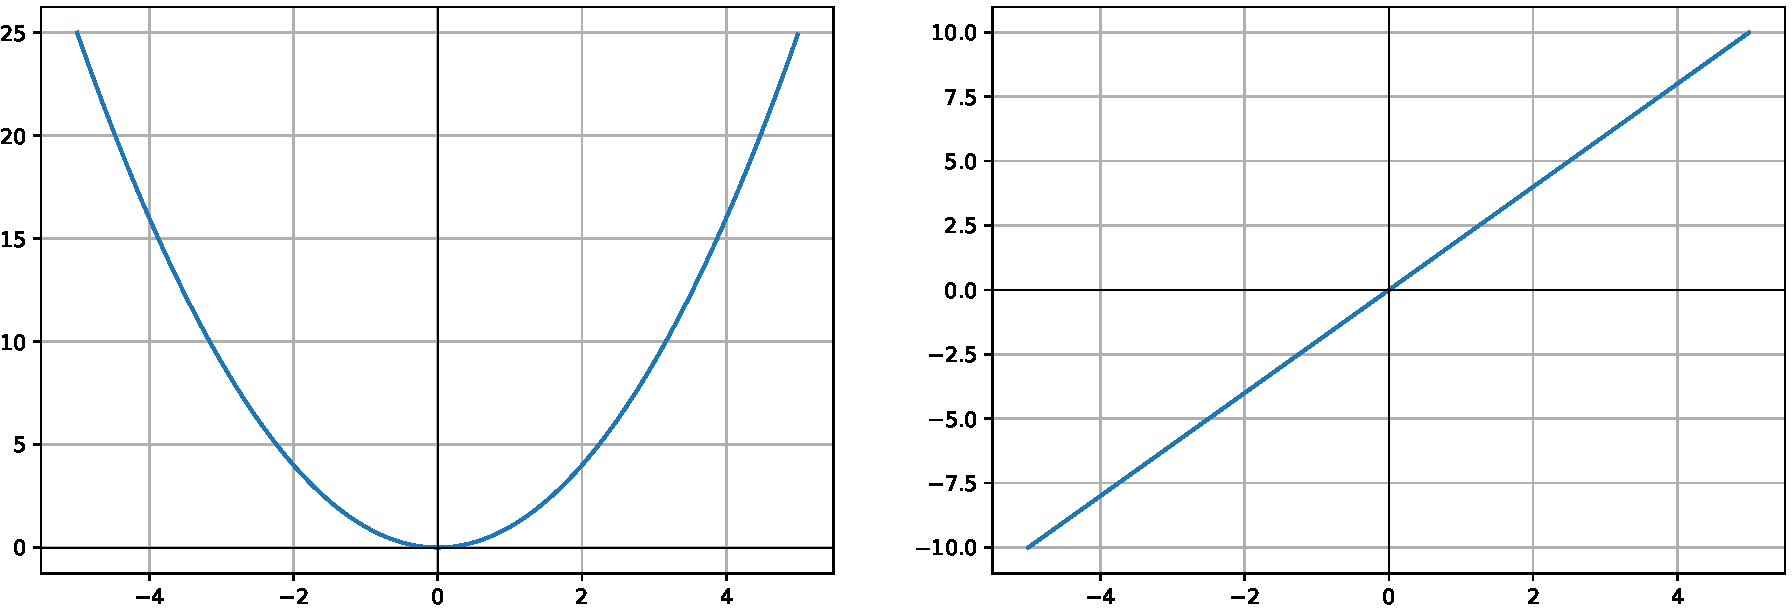
\includegraphics[width=\textwidth]{Pow2.pdf}
\centering
\caption{Parabola i njena derivacija}
\label{fig:pow2}
\end{figure}

\begin{equation}
\begin{split}
f(x) = x^2
\end{split}
\qquad
\begin{split}
f'(x) = 2x
\end{split}
\end{equation}

\todo{koji problem rješava}
\todo{svojstva}
\todo{problemi}

\subsection{Kubna parabola $x^3$}

\begin{figure}[H]
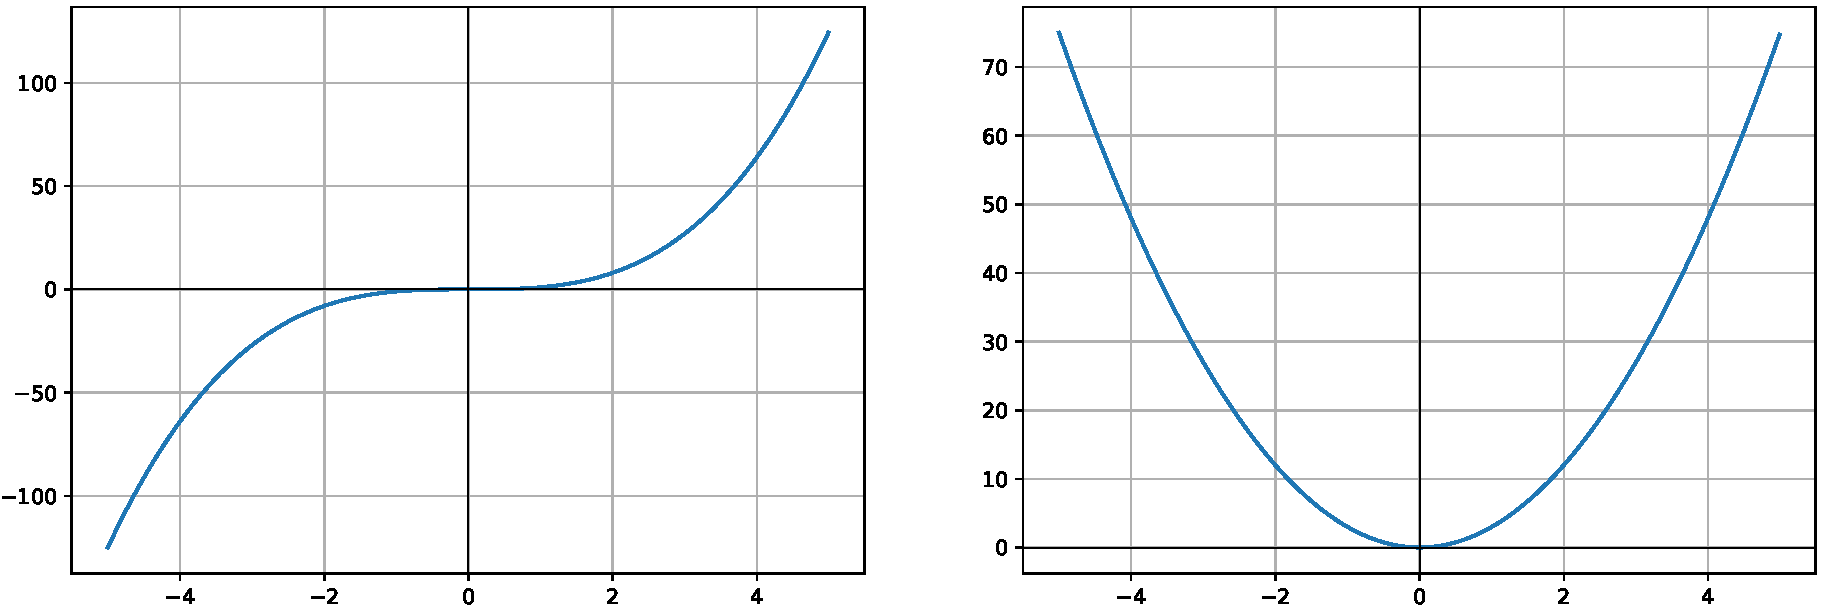
\includegraphics[width=\textwidth]{Pow3.pdf}
\centering
\caption{Kubna parabola i njena derivacija}
\label{fig:pow3}
\end{figure}

\begin{equation}
\begin{split}
f(x) = x^3
\end{split}
\qquad
\begin{split}
f'(x) = 3x^2
\end{split}
\end{equation}

\todo{koji problem rješava}
\todo{svojstva}
\todo{problemi}

\subsection{Gauss}

\begin{figure}[H]
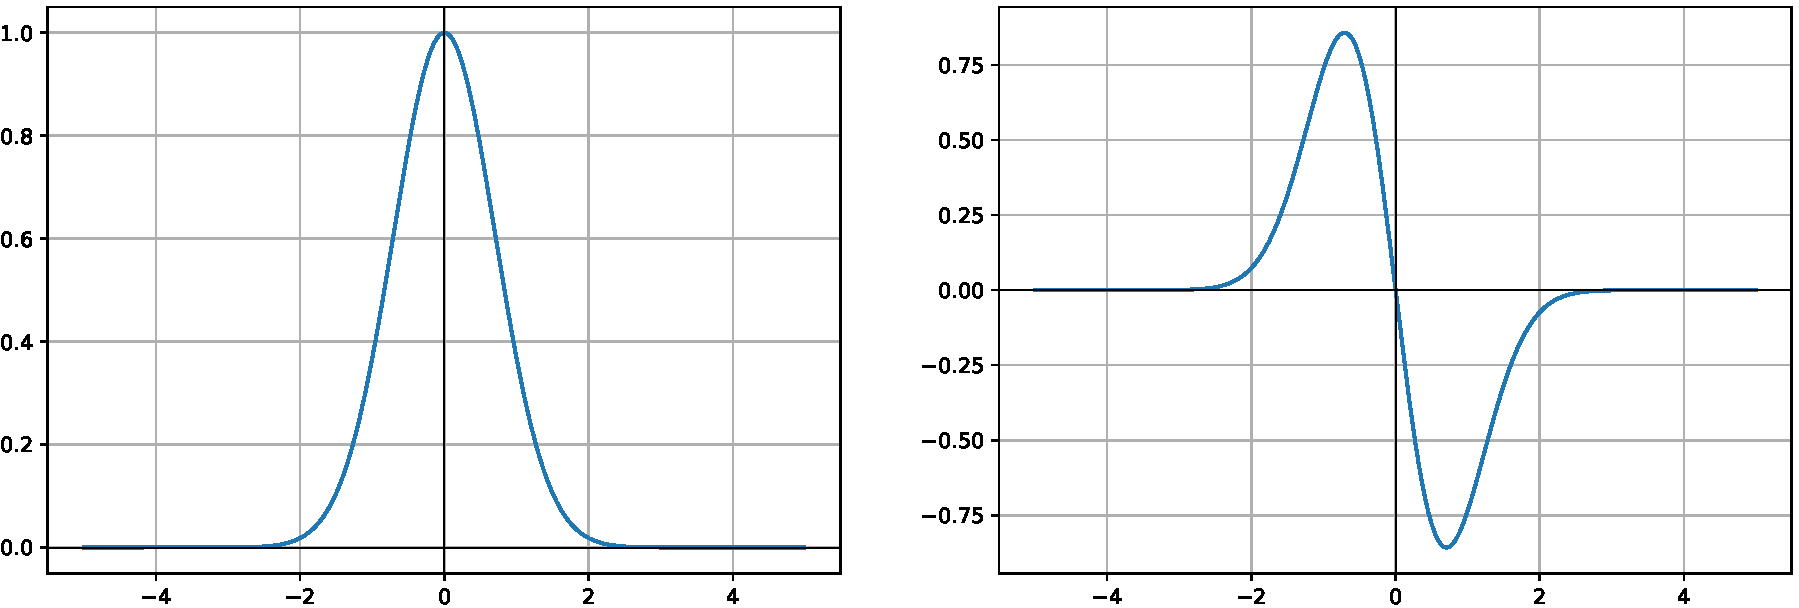
\includegraphics[width=\textwidth]{Gauss.pdf}
\centering
\caption{Gaussolika funkcija i njena derivacija}
\label{fig:gauss}
\end{figure}

\begin{equation}
\begin{split}
f(x) = e^{-x^2}
\end{split}
\qquad
\begin{split}
f'(x) = -2x \cdot f(x)
\end{split}
\end{equation}

\todo{koji problem rješava}
\todo{svojstva}
\todo{problemi}

\section{Izlazne funkcije posebne namjene}

\subsection{(DReLU)}
\engl{Dual ReLU}

\todoimg{}

\begin{equation}
???
\end{equation}

\todo{koji problem rješava}
\todo{svojstva}
\todo{problemi}

Koristi se u rekurzivnim neuronskim mrežama kako bi se 

%--------------------------------------------------------------------------------------%
\chapter{Optimizacija simboličkom regresijom (tehnički genetskim programiranjem...)}

\section{Simbolička regresija}
\todo{Opis i svojstva SR}
\todo{Utjecaj i brojnost parametara u GA (moš linkat i svoj završni rad :P)}

\subsection{Pretraživanje izlaznih funkcija}
\todo{golden activation članak, kako radi detaljnije}
\todo{swish članak detaljnije}

\subsection{Neuronska mreža kao funkcija}
\todo{Kako predstaviti čitavu mrežu grafom}
\todo{CGP Atari rad}
\todo{Spomeni da je to kao evolucija prijenosne funkcije (i ulazna i izlazna se definiraju)}

\section{Taboo evolucijski algoritam}
\todo{Problem konvergencije i stohastičnosti GP-a}
\todo{EA oplemenjen taboo listom iz algoritma Taboo pretraživanja}

\section{Korišteni čvorovi (prostor pretraživanja)}
U nastavku je dan popis čvorova koji ujedno definiraju prostor pretraživanja.

\begin{table}
\begin{tabular}[t]{lr}
\begin{tabular}[t]{l|c|r}
\textbf{Naziv} & \textbf{Funkcija} & \textbf{Broj ulaza} \\
\hline
x		& $x$					& 0 \\
const	& $c \in \realnum$		& 0 \\
\hline
+		& $x + y$				& 2 \\
-		& $x - y$				& 2 \\
*		& $x \cdot y$			& 2 \\
/		& $\frac{x}{y + 1e-12}$	& 2 \\
\hline
min		& $min(x, y)$			& 2 \\
max		& $max(x, y)$			& 2 \\
abs		& $|x|$					& 1 \\
\hline
sin		& $sin(x)$				& 1 \\
cos		& $cos(x)$				& 1 \\
tan		& $tan(x)$				& 1 \\
\hline
exp		& $e^x$					& 1 \\
log		& $log_e(x)$				& 1 \\
pow2		& $x^2$					& 1 \\
pow3		& $x^3$					& 1 \\
pow		& $x^y$					& 2 \\
\end{tabular}
& \quad
\begin{tabular}[t]{l|c|r}
\textbf{Naziv} & \textbf{Funkcija} & \textbf{Broj ulaza} \\
\hline
elu		& $ELU(x)$				& 1 \\
gauss	& $e^{x^2}$				& 1 \\
lrelu	& $LReLU(x)$				& 1 \\
relu		& $ReLU(x)$				& 1 \\
selu		& $SELU(x)$				& 1 \\
sigmoid	& $\frac{1}{1+e^{-x}}$	& 1 \\
softmax	& $Softmax(x)$			& 1 \\
sotplus	& $Softplus(x)$			& 1 \\
softsign	& $Softsign(x)$			& 1 \\
swish	& $Swish(x)$				& 1 \\
tanh		& $tanh(x)$				& 1 \\
\end{tabular}
\end{tabular}
\caption{Popis korištenih čvorova}
\end{table}

%--------------------------------------------------------------------------------------%
\chapter{Implementacija}
\section{Razvojna okolina i alati}
\todo{tulavi DL4J}
\todo{IntelliJ <3 <3 <3}
\todo{funkcije iscrtavam u jn}

\section{Parametri}
\todo{da, možeš definirat parametre u datoteki}
\todo{dodavanje parametara}
\todo{grid search mehanizam}

\section{Evolucijski algoritmi}
\todo{in-house EA okolina}
\todo{glavne komponente koda}
\todoimg{IntelliJ generirna UML paketa genetics}

\section{Neuronske mreže}
\todo{glavne komponente}
\todo{automatizirana pohrana rezultata}
\todoimg{IntelliJ generirna UML paketa neurology}

\section{Paralelizacija}
\todo{workarbiter <3}
\todo{sinkronizacija u GA i pomoćne klase/metode}

\section{Loggovi}
\todo{kaj sve imaš i kak se koristi}

%--------------------------------------------------------------------------------------%
\chapter{Rezultati}
\label{sec:rezultati}

\section{9class}

\subsection{Uobičajene izlazne funkcije}
\todo{Opis postupka pretrage}
\todo{Tablica}
\todo{Komentar}

\subsection{Utjecaj parametra veličine taboo liste}
\todo{Tablica}
\todo{Komentar}

\todoimg{boxplot}

\section{256class}

\subsection{Uobičajene izlazne funkcije}
\todo{Opis postupka pretrage}
\todo{Tablica}
\todo{Komentar}

\subsection{Utjecaj parametra veličine taboo liste}
\todo{Tablica}
\todo{Komentar}

\todoimg{boxplot}

%--------------------------------------------------------------------------------------%
\chapter{Stvari koje sam probao, ali nisu ispale korisne}
\subsubsection{Učeći parametri}
\todo{dokaz da na korištene funkcije nema utjecaja (stopi se s težinama ili biasom)}
\todo{pokazati primjer fje gdje bi se mogao koristiti}

\subsubsection{Dropout}
\todo{zahtjeva previše iteracija, što nije baš korisno u EA okruženju}
\todo{probati maxout?}

\subsubsection{Tensorflow Java API}
\todo{probo, ali je još u razvoju (puno toga je falilo)}

%--------------------------------------------------------------------------------------%
\chapter{Buduća istraživanja}
\todo{Primjena CNN na vremenskim uzorcima po uzoru na onaj rad}
\todo{Ispitivanje učinkovitosti korištene optimizacije na ostalim problemima}
\todo{Paralelna evolucija arhitekture i aktivacijskih fja \citep{cnn_evolution}}

%--------------------------------------------------------------------------------------%
\chapter{Zaključak}
\todo{Radi/Ne radi}
\todo{Pronađene zanimljivosti}
\todo{Pouka za doma}

\bibliography{literatura}
\bibliographystyle{fer}

\begin{sazetak}
Proučiti postojeće metode u izgradnji izlaznih funkcija u umjetnim neuronskim mrežama. Posebnu pažnju posvetiti evolucijskim algoritmima simboličke regresije za izgradnju ciljanih funkcija. Ustanoviti moguće nedostatke postojećih algoritama ili mogućnost poboljšanja. Primijeniti evoluirane izlazne funkcije u homogenoj ili heterogenoj umjetnoj neuronskoj mreži na skupovima DPAv2 i DPAv4 te odrediti mjere kvalitete izgrađenog klasifikatora: točnost, preciznost, odziv te F mjere. Usporediti učinkovitost ostvarenih postupaka s postojećim rješenjima iz literature. Radu priložiti izvorne tekstove programa, dobivene rezultate uz potrebna objašnjenja i korištenu literaturu.

\kljucnerijeci{Ključne riječi, odvojene zarezima.}
\end{sazetak}

\engtitle{Optimized output functions for classifiers based on artificial neural networks in the domain of implementation attacks on cryptographic devices}
\begin{abstract}
Examine existing methods in building output functions in artificial neural networks. Give special attention to evolutionary algorithms of symbolic regression for constructing target functions. Apply evolved output functions in a homogeneous or heterogeneous artificial neural network on datasets DPAv2 and DPAv4 and examine quality measures of the built classifier: accuracy, precision, recall and F measures. Compare the efficiency of acquired methods with existing solutions from the literature. Alongside thesis attach source code of programs, acquired results with necessarry discussion and literature used.

\keywords{Keywords.}
\end{abstract}

\end{document}
